\documentclass{article}


% if you need to pass options to natbib, use, e.g.:
%     \PassOptionsToPackage{numbers, compress}{natbib}
% before loading neurips_2024


% ready for submission
% \usepackage{neurips_2024}

\PassOptionsToPackage{numbers, compress}{natbib}
\usepackage[preprint]{neurips_2024}

% to compile a preprint version, e.g., for submission to arXiv, add add the
% [preprint] option:
% \usepackage[preprint]{neurips_2024}


% to compile a camera-ready version, add the [final] option, e.g.:
%     \usepackage[final]{neurips_2024}


% to avoid loading the natbib package, add option nonatbib:
%    \usepackage[nonatbib]{neurips_2024}


\usepackage[utf8]{inputenc} % allow utf-8 input
\usepackage[T1]{fontenc}    % use 8-bit T1 fonts
\usepackage[colorlinks,
            linkcolor=red,
            anchorcolor=blue,
            citecolor=green
            ]{hyperref}
\usepackage{url}            % simple URL typesetting
\usepackage{booktabs}       % professional-quality tables
\usepackage{amsfonts}       % blackboard math symbols
\usepackage{nicefrac}       % compact symbols for 1/2, etc.
\usepackage{microtype}      % microtypography
\usepackage{xcolor}         % colors
\usepackage{caption}
\usepackage{subcaption}
\usepackage{natbib}
\usepackage{graphicx}
\usepackage{enumitem}
\usepackage{makecell}
\usepackage{amsmath}
\usepackage{amsthm}
\usepackage{thmtools}
\usepackage{thm-restate}
\usepackage{algorithm}
\usepackage{algorithmic}
\usepackage{bbm}
\usepackage{tabularx}
\usepackage{listings}
\usepackage{xcolor}
\usepackage{multirow}
\usepackage{multicol}
\usepackage{tcolorbox}
\usepackage{tikz}
\usepackage{footnote}
\usepackage{wrapfig}

% Tableau colors
\definecolor{tblue}{RGB}{31,119,180}
\definecolor{torange}{RGB}{255,127,14}
\definecolor{tgreen}{RGB}{44,160,44}
\definecolor{tred}{RGB}{214,39,40}
\definecolor{tpurple}{RGB}{148,103,189}
\definecolor{lightblue}{RGB}{173, 216, 230}
\definecolor{lightpink}{RGB}{255, 182, 193}
\definecolor{lightgreen}{RGB}{144, 238, 144}

\usepackage{colortbl}
\usepackage{xcolor}
\usepackage{array}

\newcommand{\hide}[1]{} %hide
\newcommand{\vpara}[1]{\vspace{0.05in}\noindent\textbf{#1 }}
\newcommand{\noind}[1]{\hspace{-0.05in}\noindent{#1}}
\newcommand{\etal}{\textit{et al}.}
\newcommand{\beq}[1]{\vspace{-0.03in}\begin{equation}#1\end{equation}\vspace{-0.02in}}
\newcommand{\beqn}[1]{\vspace{-0.03in}\begin{eqnarray}#1\end{eqnarray}\vspace{-0.03in}}
\newcommand{\besp}[1]{\begin{split}#1\end{split}}
\newcommand{\red}[1]{{\color{red}#1}}
\newcommand{\ie}{\textit{i}.\textit{e}.}
\newcommand{\eg}{\textit{e}.\textit{g}.} 
\newcommand{\wrt}{\textit{w}.\textit{r}.\textit{t}} 

\def\model{VideoRAG}

\title{VideoRAG: Retrieval-Augmented Generation with Extreme Long-Context Videos}


% The \author macro works with any number of authors. There are two commands
% used to separate the names and addresses of multiple authors: \And and \AND.
%
% Using \And between authors leaves it to LaTeX to determine where to break the
% lines. Using \AND forces a line break at that point. So, if LaTeX puts 3 of 4
% authors names on the first line, and the last on the second line, try using
% \AND instead of \And before the third author name.


\author{
  Xubin Ren\textsuperscript{1}\thanks{Equal contribution.}\footnotemark[1] ~~~
  Lingrui Xu\textsuperscript{1}\footnotemark[1] ~~~
  Long Xia\textsuperscript{2} ~~~
  Shuaiqiang Wang\textsuperscript{2} ~~~
  Dawei Yin\textsuperscript{2} ~~~
  Chao Huang\textsuperscript{1}\thanks{Chao Huang is the Corresponding Author.} \\
  \textsuperscript{1}The University of Hong Kong ~~~
  \textsuperscript{2}Baidu Inc. \\
  \texttt{\{xubinrencs, lingruixu.db, long.phil.xia, chaohuang75\}@gmail.com} \\
  \texttt{wangshuaiqiang@baidu.com yindawei@acm.org}
}

\begin{document}

\maketitle

\begin{abstract}
Retrieval-Augmented Generation (RAG) has demonstrated remarkable success in enhancing Large Language Models (LLMs) through external knowledge integration, yet its application has primarily focused on textual content, leaving the rich domain of multi-modal video knowledge predominantly unexplored. This paper introduces \model, the first retrieval-augmented generation framework specifically designed for processing and understanding extremely long-context videos. Our core innovation lies in its dual-channel architecture that seamlessly integrates (i) graph-based textual knowledge grounding for capturing cross-video semantic relationships, and (ii) multi-modal context encoding for efficiently preserving visual features. This novel design empowers \model\ to process unlimited-length videos by constructing precise knowledge graphs that span multiple videos while maintaining semantic dependencies through specialized multi-modal retrieval paradigms. Through comprehensive empirical evaluation on our proposed LongerVideos benchmark-comprising over 160 videos totaling 134+ hours across lecture, documentary, and entertainment categories-\model\ demonstrates substantial performance compared to existing RAG alternatives and long video understanding methods. The source code of \model\ implementation and the benchmark dataset are openly available at: \textcolor{blue}{\url{https://github.com/HKUDS/VideoRAG}}.
\end{abstract}

% \clearpage

\section{Introduction}


\begin{figure}[t]
\centering
\includegraphics[width=0.6\columnwidth]{figures/evaluation_desiderata_V5.pdf}
\vspace{-0.5cm}
\caption{\systemName is a platform for conducting realistic evaluations of code LLMs, collecting human preferences of coding models with real users, real tasks, and in realistic environments, aimed at addressing the limitations of existing evaluations.
}
\label{fig:motivation}
\end{figure}

\begin{figure*}[t]
\centering
\includegraphics[width=\textwidth]{figures/system_design_v2.png}
\caption{We introduce \systemName, a VSCode extension to collect human preferences of code directly in a developer's IDE. \systemName enables developers to use code completions from various models. The system comprises a) the interface in the user's IDE which presents paired completions to users (left), b) a sampling strategy that picks model pairs to reduce latency (right, top), and c) a prompting scheme that allows diverse LLMs to perform code completions with high fidelity.
Users can select between the top completion (green box) using \texttt{tab} or the bottom completion (blue box) using \texttt{shift+tab}.}
\label{fig:overview}
\end{figure*}

As model capabilities improve, large language models (LLMs) are increasingly integrated into user environments and workflows.
For example, software developers code with AI in integrated developer environments (IDEs)~\citep{peng2023impact}, doctors rely on notes generated through ambient listening~\citep{oberst2024science}, and lawyers consider case evidence identified by electronic discovery systems~\citep{yang2024beyond}.
Increasing deployment of models in productivity tools demands evaluation that more closely reflects real-world circumstances~\citep{hutchinson2022evaluation, saxon2024benchmarks, kapoor2024ai}.
While newer benchmarks and live platforms incorporate human feedback to capture real-world usage, they almost exclusively focus on evaluating LLMs in chat conversations~\citep{zheng2023judging,dubois2023alpacafarm,chiang2024chatbot, kirk2024the}.
Model evaluation must move beyond chat-based interactions and into specialized user environments.



 

In this work, we focus on evaluating LLM-based coding assistants. 
Despite the popularity of these tools---millions of developers use Github Copilot~\citep{Copilot}---existing
evaluations of the coding capabilities of new models exhibit multiple limitations (Figure~\ref{fig:motivation}, bottom).
Traditional ML benchmarks evaluate LLM capabilities by measuring how well a model can complete static, interview-style coding tasks~\citep{chen2021evaluating,austin2021program,jain2024livecodebench, white2024livebench} and lack \emph{real users}. 
User studies recruit real users to evaluate the effectiveness of LLMs as coding assistants, but are often limited to simple programming tasks as opposed to \emph{real tasks}~\citep{vaithilingam2022expectation,ross2023programmer, mozannar2024realhumaneval}.
Recent efforts to collect human feedback such as Chatbot Arena~\citep{chiang2024chatbot} are still removed from a \emph{realistic environment}, resulting in users and data that deviate from typical software development processes.
We introduce \systemName to address these limitations (Figure~\ref{fig:motivation}, top), and we describe our three main contributions below.


\textbf{We deploy \systemName in-the-wild to collect human preferences on code.} 
\systemName is a Visual Studio Code extension, collecting preferences directly in a developer's IDE within their actual workflow (Figure~\ref{fig:overview}).
\systemName provides developers with code completions, akin to the type of support provided by Github Copilot~\citep{Copilot}. 
Over the past 3 months, \systemName has served over~\completions suggestions from 10 state-of-the-art LLMs, 
gathering \sampleCount~votes from \userCount~users.
To collect user preferences,
\systemName presents a novel interface that shows users paired code completions from two different LLMs, which are determined based on a sampling strategy that aims to 
mitigate latency while preserving coverage across model comparisons.
Additionally, we devise a prompting scheme that allows a diverse set of models to perform code completions with high fidelity.
See Section~\ref{sec:system} and Section~\ref{sec:deployment} for details about system design and deployment respectively.



\textbf{We construct a leaderboard of user preferences and find notable differences from existing static benchmarks and human preference leaderboards.}
In general, we observe that smaller models seem to overperform in static benchmarks compared to our leaderboard, while performance among larger models is mixed (Section~\ref{sec:leaderboard_calculation}).
We attribute these differences to the fact that \systemName is exposed to users and tasks that differ drastically from code evaluations in the past. 
Our data spans 103 programming languages and 24 natural languages as well as a variety of real-world applications and code structures, while static benchmarks tend to focus on a specific programming and natural language and task (e.g. coding competition problems).
Additionally, while all of \systemName interactions contain code contexts and the majority involve infilling tasks, a much smaller fraction of Chatbot Arena's coding tasks contain code context, with infilling tasks appearing even more rarely. 
We analyze our data in depth in Section~\ref{subsec:comparison}.



\textbf{We derive new insights into user preferences of code by analyzing \systemName's diverse and distinct data distribution.}
We compare user preferences across different stratifications of input data (e.g., common versus rare languages) and observe which affect observed preferences most (Section~\ref{sec:analysis}).
For example, while user preferences stay relatively consistent across various programming languages, they differ drastically between different task categories (e.g. frontend/backend versus algorithm design).
We also observe variations in user preference due to different features related to code structure 
(e.g., context length and completion patterns).
We open-source \systemName and release a curated subset of code contexts.
Altogether, our results highlight the necessity of model evaluation in realistic and domain-specific settings.





% Consider a lasso optimization procedure with potentially distinct regularization penalties:
% \begin{align}
%     \hat{\beta} = \arg\min_{\beta}\{\|y-X\beta\|^2_2+\sum_{i=1}^{N}\lambda_i|\beta_i|\}.
% \end{align}
\subsection{Supervised Data-Driven Learning}\label{subsec:supervised}
We consider a generic data-driven supervised learning procedure. Given a dataset \( \mathcal{D} \) consisting of \( n \) data points \( (x_i, y_i) \in \mathcal{X} \times \mathcal{Y} \) drawn from an underlying distribution \( p(\cdot|\theta) \), our goal is to estimate parameters \( \theta \in \Theta \) through a learning procedure, defined as \( f: (\mathcal{X} \times \mathcal{Y})^n \rightarrow \Theta \) 
that minimizes the predictive error on observed data. 
Specifically, the learning objective is defined as follows:
\begin{align}
\hat{\theta}_f := f(\mathcal{D}) = \arg\min_{\theta} \mathcal{L}(\theta, \mathcal{D}),
\end{align}
where \( \mathcal{L}(\cdot,\mathcal{D}) := \sum_{i=1}^{n} \mathcal{L}(\cdot, (x_i, y_i))\), and $\mathcal{L}$ is a loss function quantifying the error between predictions and true outcomes. 
Here, $\hat{\theta}_f$ is the parameter that best explains the observed data pairs \( (x_i, y_i) \) according to the chosen loss function \( \mathcal{L} (\cdot) \).

\paragraph{Feature Selection.}
Feature selection aims to improve model \( f \)'s predictive performance while minimizing redundancy. 
%Formally, given data \( X \), response \( y \), feature set \( \mathcal{F} \), loss function \( \mathcal{L}(\cdot) \), and a feature limit \( k \), the objective is:
% \begin{align}
% \mathcal{S}^* = \arg \min_{\mathcal{S} \subseteq \mathcal{F}, |\mathcal{S}| \leq k} \mathcal{L}(y, f(X_\mathcal{S})) + \lambda R(\mathcal{S}),
% \end{align}
% where \( X_\mathcal{S} \) is the submatrix of \( X \) for selected features \( \mathcal{S} \), \( \lambda \) is a regularization parameter, and \( R(\mathcal{S}) \) penalizes feature redundancy.
 State-of-the-art techniques fall into four categories: (i) filter methods, which rank features based on statistical properties like Fisher score \citep{duda2001pattern,song2012feature}; (ii) wrapper methods, which evaluate model performance on different feature subsets \citep{kohavi1997wrappers}; (iii) embedded methods, which integrate feature selection into the learning process using techniques like regularization \citep{tibshirani1996LASSO,lemhadri2021lassonet}; and (iv) hybrid methods, which combine elements of (i)-(iii) \citep{SINGH2021104396,li2022micq}. This paper focuses on embedded methods via Lasso, benchmarking against approaches from (i)-(iii).

\subsection{Language Modeling}
% The objective of language modeling is to learn a probability distribution \( p_{LM}(x) \) over sequences of text \( x = (X_1, \ldots, X_{|x|}) \), such that \( p_{LM}(x) \approx p_{text}(x) \), where \( p_{text}(x) \) represents the true distribution of natural language. This process involves estimating the likelihood of token sequences across variable lengths and diverse linguistic structures.
% Modern large language models (LLMs) are trained on vast datasets spanning encyclopedias, news, social media, books, and scientific papers \cite{gao2020pile}. This broad training enables them to generalize across domains, learn contextual knowledge, and perform zero-shot learning—tackling new tasks using only task descriptions without fine-tuning \cite{brown2020gpt3}.
Language modeling aims to approximate the true distribution of natural language \( p_{\text{text}}(x) \) by learning \( p_{\text{LM}}(x) \), a probability distribution over text sequences \( x = (X_1, \ldots, X_{|x|}) \). Modern large language models, trained on diverse datasets \citep{gao2020pile}, exhibit strong generalization across domains, acquire contextual knowledge, and perform zero-shot learning—solving new tasks using only task descriptions—or few-shot learning by leveraging a small number of demonstrations \citep{brown2020gpt3}.
\paragraph{Retrieval-Augmented Generation (RAG).} Retrieval-Augmented Generation (RAG) enhances the performance of generative language models by  integrating a domain-specific information retrieval process  \citep{lewis2020retrieval}. The RAG framework comprises two main components: \textit{retrieval}, which extracts relevant information from external knowledge sources, and \textit{generation}, where an LLM generates context-aware responses using the prompt combined with the retrieved context. Documents are indexed through various databases, such as relational, graph, or vector databases \citep{khattab2020colbert, douze2024faiss, peng2024graphretrievalaugmentedgenerationsurvey}, enabling efficient organization and retrieval via algorithms like semantic similarity search to match the prompt with relevant documents in the knowledge base. RAG has gained much traction recently due to its demonstrated ability to reduce incidence of hallucinations and boost LLMs' reliability as well as performance \citep{huang2023hallucination, zhang2023merging}. 
 
% image source: https://medium.com/@bindurani_22/retrieval-augmented-generation-815c1ae438d8
\begin{figure}
    \centering
\includegraphics[width=1.03\linewidth]{fig/fig1.pdf}
\vspace{-0.6cm}
\scriptsize 
    \caption{Retrieval Augmented Generation (RAG) based $\ell_1$-norm weights (penalty factors) for Lasso. Only feature names---no training data--- are included in LLM prompt.} 
    \label{fig:rag}
\end{figure}
% However, for the RAG model to be effective given the input token constraints of the LLM model used, we need to effectively process the retrieval documents through a procedure known as \textit{chunking}.

\subsection{Task-Specific Data-Driven Learning}
LLM-Lasso aims to bridge the gap between data-driven supervised learning and the predictive capabilities of LLMs trained on rich metadata. This fusion not only enhances traditional data-driven methods by incorporating key task-relevant contextual information often overlooked by such models, but can also be especially valuable in low-data regimes, where the learning algorithm $f:\mathcal{D}\rightarrow\Theta$ (seen as a map from datasets $\mathcal{D}$ to the space of decisions $\Theta$) is susceptible to overfitting.

The task-specific data-driven learning model $\tilde{f}:\mathcal{D}\times\mathcal{D}_\text{meta}\rightarrow\Theta$ can be described as a metadata-augmented version of $f$, where a link function $h(\cdot)$ integrates metadata (i.e. $\mathcal{D}_\text{meta}$) to refine the original learning process. This can be expressed as:
\[
\tilde{f}(\mathcal{D}, \mathcal{D}_\text{meta}) := \mathcal{T}(f(\mathcal{D}),  h(\mathcal{D}_{\text{meta}})),
\]
where the functional $\mathcal{T}$ takes the original learning algorithm $f(\mathcal{D})$ and transforms it into a task-specific learning algorithm $\tilde{f}(\mathcal{D}, \mathcal{D}_\text{meta})$ by incorporating the metadata $\mathcal{D}_\text{meta}$. 
% In particular, the link function $h(\mathcal{D}_{\text{meta}})$ provides a structured mechanism summarizing the contextual knowledge.

There are multiple approaches to formulate $\mathcal{T}$ and $h$.
%to ``inform" the data-driven model $f$ of %meta knowledge. 
For instance, LMPriors \citep{choi2022lmpriorspretrainedlanguagemodels} designed $h$ and $\mathcal{T}$ such that $h(\mathcal{D}_{\text{meta}})$ first specifies which features to retain (based on a probabilistic prior framework), and then $\mathcal{T}$ keeps the selected features and removes all the others from the original learning objective of $f$. 
Note that this approach inherently is restricted as it selects important features solely based on $\mathcal{D}_\text{meta}$ without seeing $\mathcal{D}$.

In contrast, we directly embed task-specific knowledge into the optimization landscape through regularization by introducing a structured inductive bias. This bias guides the learning process toward solutions that are consistent with metadata-informed insights, without relying on explicit probabilistic modeling. Abstractly, this can be expressed as:
\begin{align}
    \!\!\!\!\!\hat{\theta}_{\tilde{f}} := \tilde{f}(\mathcal{D},\mathcal{D}
    _\text{meta})= \arg\min_{\theta} \mathcal{L}(\theta, \mathcal{D}) + \lambda R(\theta, \mathcal{D}_{\text{meta}}),
\end{align}
where \( \lambda \) is a regularization parameter, \( R(\cdot) \) is a regularizer, and $\theta$ is the prediction parameter.
%We explain our framework with more details in the following section.


% Our research diverges from both aforementioned approaches by positioning the LLM not as a standalone feature selector but as an enhancement to data-driven models through an embedded feature selection method, L-LASSO. L-LASSO incorporates domain expertise—auxiliary natural language metadata about the task—via the LLM-informed LASSO penalty, which is then used in statistical models to enhance predictive performance. This method integrates the rich, context-sensitive insights of LLMs with the rigor and transparency of statistical modeling, bridging the gap between data-driven and knowledge-driven feature selection approaches. To approach this task, we need to tackle two key components: (i). train an LLM that is expert in the task-specific knowledge; (ii). inform data-driven feature selector LASSO with LLM knowledge.

% In practice, this involves combining techniques like prompt engineering and data engineering to develop an effective framework for integrating metadata into existing data-driven models. We will go through this in detail in Section \ref{mthd} and \ref{experiment}.


\section{The \model\ Framework}

\begin{figure*}[t]
    \centering
    \includegraphics[width=1.0\textwidth]{figs/framework.pdf}
    \vspace{-0.2in}
    \caption{The overall framework of our proposed RAG framework \model\ for videos.}
    \vspace{-0.1in}
    \label{fig:framework}
\end{figure*}

We present our retrieval-augmented generation framework designed for understanding unlimited-length video content. Our approach addresses two fundamental challenges: (1) multi-modal knowledge indexing that effectively captures and organizes visual, audio, and semantic information from videos, and (2) knowledge-grounded information retrieval that enables precise retrieval of relevant video clips for generating accurate responses through large language models. In the following sections, we detail these components and their integration into a unified video understanding system.

\subsection{Multi-Modal Video Knowledge Indexing}



Unlike traditional text documents, videos encapsulate information through multiple modalities - primarily visual frames - creating unique challenges for knowledge extraction and organization. Standard text-based RAG methods prove insufficient for video content due to several fundamental limitations: (1) text-based systems cannot directly capture visual dynamics; (2) temporal dependencies that traditional RAG approaches fail to preserve across video frames; (3) cross-modal interactions that simple text encoding cannot capture between visual and textual information. 

To address these challenges, we introduce a comprehensive indexing framework with two components: \textbf{Graph-based Textual Knowledge Grounding} that transforms multi-modal signals into structured textual representations while preserving semantic relationships and temporal dependencies, and \textbf{Multi-Modal Context Encoding} that captures fine-grained cross-modal interactions through unified embeddings. This dual-channel architecture enables \model\ to effectively organize and index long-context videos while preserving the semantic richness of multi-modal content.

\subsubsection{\textbf{Graph-based Textual Knowledge Grounding}}
\label{sec:textual indexing}

Our framework transforms multi-modal video content into structured textual knowledge through graph-based techniques for enhanced indexing and retrieval. The conversion process operates across two key modalities: for visual content, we employ state-of-the-art Vision Language Models (VLMs) to generate comprehensive textual descriptions capturing scene dynamics and contextual information; for auditory streams, we leverage high-fidelity Automatic Speech Recognition (ASR) to extract spoken content with temporal alignment. This dual-stream processing ensures both visual semantics and audio information are preserved in our textual knowledge representation.

\begin{itemize}[leftmargin=*]
    \item \textbf{Vision-Text Grounding}: To analyze visual content effectively, we segment each video $\mathcal{V}$ into short clips ${\mathcal{S}_1, \ldots, \mathcal{S}_m}$, enabling processing of unlimited-length videos. For each clip $\mathcal{S}_j$, we transform visual information into text through a two-step process: first, we uniformly sample $k$ frames ($k \leq 10$) chronologically to capture key visual elements; then, we employ Vision-Language Models (VLMs) to generate comprehensive natural language descriptions capturing objects, actions, and scene dynamics. The caption generation process follows:
    \begin{align}
        \mathcal{C}_j = \text{VLM}(\mathcal{T}_j, \{\textbf{F}_1, \ldots, \textbf{F}_k\} \mid \textbf{F} \in \mathcal{S}_j),
    \end{align}
    where ${\textbf{F}}$ denotes the chronologically ordered set of $k$ sampled frames from the clip $\mathcal{S}_j$. We maintain $k \leq 10$ to optimize efficiency while preserving temporal coherence. The model integrates both visual frames and clip transcript $\mathcal{T}_j$ as input prompts, enabling the VLM to generate contextually rich captions $\mathcal{C}_j$ that capture both visual dynamics and associated speech content.
    
    \item \textbf{Audio-Text Grounding}: To capture crucial elements like dialogue and narration that enrich video understanding, we employ Automatic Speech Recognition (ASR) technology to transcribe each video clip, where $\mathcal{T}_j = \text{ASR}(\mathcal{S}_j)$ represents the extracted transcript from the clip $\mathcal{S}_j$.
\end{itemize}


For each video clip $\mathcal{S}$, we then create a unified and semantically rich textual representation by systematically merging the generated visual captions and ASR transcriptions $(\mathcal{C}, \mathcal{T})$. For a video $\mathcal{V}$ containing $m$ sequential clips, we formalize the complete knowledge extraction process as:
\begin{align}
    \mathcal{V}^{t} = \{(\mathcal{C}_l, \mathcal{T}_l) \mid l \in [1, m]\}.
\end{align}
At the core of our \model\ lies the challenge of organizing and retrieving multi-video knowledge efficiently. To address this, we propose a graph-based indexing framework that systematically links textual knowledge across different videos. This architecture enables incremental construction of a comprehensive knowledge graph from the extracted textual information, while maintaining semantic relationships and contextual dependencies. The entire process is executed through these essential steps, each designed to optimize multi-modal knowledge representation and retrieval:
\begin{itemize}[leftmargin=*]
    \item \textbf{Semantic Entity Recognition and Relationship Mapping}:
    Our framework leverages Large Language Models (LLMs) to construct a high-quality knowledge graph $\mathcal{G} = (\mathcal{N}, \mathcal{E})$ that comprehensively captures and connects video knowledge. To optimize LLM performance and manage their context window limitations effectively, we implement a strategic processing pipeline: \\\vspace{-0.12in}
    
    $\bullet$ (i) \textbf{Text Segmentation}. The first stage focuses on text segmentation, where we methodically divide video textual descriptions $\mathcal{V}^{t}$ into manageable chunks $\mathcal{H}_i \in \mathcal{V}^{t}$. Each chunk is carefully constructed to contain multiple video clip descriptions while adhering to a predefined length threshold, ensuring optimal processing while maintaining semantic coherence. \\\vspace{-0.12in}

    $\bullet$ (ii) \textbf{Entity-Relation Extraction}. In the entity-relation extraction phase, we process each chunk's caption-transcript pairs through LLMs to identify key entities (represented as nodes $\mathcal{N}$) and extract meaningful relationships (represented as edges $\mathcal{E}$). For instance, given the text ``\textit{GPT-4 utilizes transformer architecture for advanced natural language understanding, while incorporating visual features through ViT's patch-based image encoding}'', the system extracts entities ``\textit{GPT-4}'', ``\textit{transformer architecture}'', and ``\textit{Vision Transformer (ViT)}'', along with relationships ``\textit{GPT-4 utilizes transformer architecture}'' and ``\textit{GPT-4 incorporates ViT's encoding}'' in the domain of LLMs.

    \item \textbf{Incremental Graph Construction and Cross-Video Knowledge Integration}:
    The construction of our comprehensive knowledge graph follows an iterative and systematic approach across multiple video sources. Our framework implements a sophisticated incremental construction process that ensures coherent knowledge integration through several key mechanisms:

    $\bullet$ (i) \textbf{Entity Unification and Merging}. Our cross-video entity unification process systematically identifies and merges semantically equivalent entities across various videos into unified nodes within the knowledge graph $\mathcal{G}$. This unification approach not only maintains a consistent representation of entities but also preserves the rich contextual information derived from diverse video sources. As a result, it effectively creates a cohesive and interconnected knowledge network that enhances the overall understanding and usability of the information contained within the graph. \\\vspace{-0.12in}

    $\bullet$ (ii) \textbf{Dynamic Knowledge Graph Evolution}. As new video content is processed, our knowledge graph undergoes systematic expansion through dual-track evolution: the integration of newly discovered entities and the establishment of previously unobserved relationships. When processing textual chunks from incoming videos, the system not only identifies and incorporates novel entities (e.g., emerging AI architectures or methodologies) but also discovers new semantic connections between existing nodes. This bidirectional growth process simultaneously reinforces established knowledge patterns while accommodating emerging concepts, ensuring the graph maintains both comprehensiveness and adaptability as it scales. \\\vspace{-0.12in}

    $\bullet$ (iii) \textbf{LLM-Powered Semantic Synthesis}. To maintain semantic coherence, we strategically leverage Large Language Models (LLMs) to generate unified entity descriptions by synthesizing information from multiple video clips. This synthesis process ensures each entity maintains a comprehensive yet consistent representation, effectively consolidating knowledge across different video contexts while preserving semantic accuracy throughout the knowledge structure. \\\vspace{-0.12in}

    Formally, we define the construction of our complete knowledge graph as follows:
    \begin{align}
        \mathcal{G} = (\mathcal{N}, \mathcal{E}) = \bigcup_{\mathcal{H} \in \{ \mathcal{V}_{1}^{t}, \ldots, \mathcal{V}_{n}^{t} \}} (\mathcal{N}_{\mathcal{H}}, \mathcal{E}_{\mathcal{H}}),
    \end{align}
    Let $(\mathcal{N}_{\mathcal{H}}, \mathcal{E}_{\mathcal{H}})$ denote the extracted entities and their relations from each text chunk $\mathcal{H}$, split from the video description $\mathcal{V}^{t}$. Through processing of all videos, we construct the complete graph $\mathcal{G}$.

    \item \textbf{Text Chunk Embedding}. For each text chunk $\mathcal{H}$, we encode a text embedding $\mathbf{e}_{\mathcal{H}}^{t} = \text{TEnc}(\mathcal{H})$ using a text encoder $\text{TEnc}(\cdot)$, enabling efficient retrieval of raw chunks. We denote the complete set of chunks as $H$ and represent their collective text embeddings as $\mathbf{E}_{H}^{t} \in \mathbb{R}^{|H| \times d_{t}}$, where $|H|$ represents the total chunk count and $d_{t}$ denotes the embedding dimension. The knowledge graph $\mathcal{G}$ and chunk embeddings $\mathbf{E}_{H}^{t}$ together form the core components of our graph indexing module.
\end{itemize}

\subsubsection{Multi-Modal Context Encoding}
\label{sec:visual indexing}

In vision-to-text grounding, certain visual nuances are inherently lost, such as lighting dynamics and intricate object details that resist accurate textual representation. To preserve these visual elements, we employ a multi-modal encoder $\text{MEnc}(\cdot)$ that transforms video content into retrieval-optimized embeddings. This encoder is capable of mapping both visual content and textual queries into a shared feature space, enabling efficient semantic retrieval. Building upon powerful multi-modal encoding frameworks like CLIP~\citep{CLIP} and ImageBind~\citep{Imgebind}, we formalize our video encoding as:
\begin{align}
    \mathbf{E}_{S}^{v} \in \mathbb{R}^{|S| \times d_{v}} \quad \textit{w.r.t.} \quad \textbf{e}_{\mathcal{S}}^{v} = \text{MEnc}(\mathcal{S}).
\end{align}
In this formulation, each video clip $\mathcal{S}$ is encoded into an embedding, collectively forming $\mathbf{E}_{S}^{v}$. Here, we utilize the capital $S$ to represent the complete clip set, with $|S|$ denoting the total clip count and $d_{v}$ representing the visual embedding dimensionality. Our \model\ framework's indexing module $\varphi(\cdot)$ processes the video knowledge base $\mathcal{D} = {\mathcal{V}_1, \ldots, \mathcal{V}_n}$ to create a hybrid index combining both knowledge graph and multi-modal context embeddings:
\begin{align}
    \hat{\mathcal{D}} = \varphi(\mathcal{D}) = (\mathcal{G}, \mathbf{E}_{H}^{t}, \mathbf{E}_{S}^{v}).
\end{align}

\subsection{Multi-Modal Retrieval Paradigm}

The Multi-Modal Retrieval Paradigm aims to efficiently retrieve relevant knowledge from videos in response to queries by integrating both textual semantic and visual content matching. Leveraging a hybrid indexing framework $\hat{\mathcal{D}}$, this approach identifies informative video clips and generates query-specific descriptions using VLMs, ensuring a comprehensive retrieval process that captures both semantic understanding and visual context for more accurate responses.
\begin{itemize}[leftmargin=*]
    \item \textbf{Textual Semantic Matching}. The textual retrieval process leverages our constructed knowledge graph $\mathcal{G}$, where each entity contains a text description derived from relevant text chunks. The retrieval process consists of four sequential steps: (i) \textbf{Query Reformulation}: In the initial step, we employ LLMs to reformulate the input query into a declarative sentence, optimizing it for subsequent entity matching operations. (ii) \textbf{Entity Matching}: The system then calculates similarity scores between this reformulated query and entity descriptions within the knowledge graph, identifying the most relevant entities along with their associated text chunks. (iii) \textbf{Chunk Selection}: Following entity matching, we apply a GraphRAG~\cite{GraphRAG}-based methodology to sort and identify the most pertinent chunks ${\mathcal{H}}_{q}$ from the retrieved collection. (iv) \textbf{Video Clip Retrieval}: Finally, we extract video clips from the selected chunks, as each chunk contains descriptions of multiple video clips, resulting in our final textual retrieval set ${\mathcal{S}}_{q}^{t}$.    
    
    \item \textbf{Visual Retrieval via Content Embeddings}. Our framework complements textual matching with direct visual retrieval, enabling semantic alignment between queries and video clips. Building upon our established visual indexing framework (Section~\ref{sec:visual indexing}), each video clip is encoded through a multi-modal encoder $\text{MEnc}(\cdot)$ to generate content-based embeddings. The visual retrieval process operates in two stages: (i) \textbf{Scene Information Extraction from Query:} We leverage LLMs to distill the query $q$ into its core visual scene components, creating a focused scene description. For instance: Original question: ``\emph{In the movie, what color is the car that chases the main character through the city?}''; Scene-focused reformulation: ``\emph{An intense urban chase sequence featuring a car pursuing someone through city streets, with buildings and traffic in the background}'' (ii) \textbf{Cross-Modal Feature Alignment:} This scene-centric query reformulation is projected into the same feature space as our visual embeddings using the multi-modal encoder, leveraging its cross-modal capabilities~\cite{CLIP,Imgebind} to align the context from different modalities. We compute similarity scores between the query embedding and video clip embeddings $\mathbf{E}_{S}^{v}$ through cosine similarity, denoted as $\text{Sim}(\text{MEnc}(q), \mathbf{E}_{S}^{v})$. The top-K matching clips form the visual retrieval result ${\mathcal{S}}_{q}^{v}$.
    
    \item \textbf{LLMs-based Video Clip Filtering}: To filter out noisy clips from the retrieved results, we employ LLMs to evaluate each clip $\mathcal{S} \in {\mathcal{S}}_{q}^{t} \cap {\mathcal{S}}_{q}^{v}$ for its relevance to query $q$ using textual and visual information $\mathcal{V}^{t}_{\mathcal{S}}$ (Section~\ref{sec:textual indexing}). The filtered clips are formally defined as:
    \begin{align}
        \{\hat{\mathcal{S}} \mid (\hat{\mathcal{S}} \in \{\mathcal{S}\}_{q}^{t} \cap \{\mathcal{S}\}_{q}^{v}) \land  \text{LLMs-Judge}(\mathcal{V}^{t}_{\hat{\mathcal{S}}}) = 1\},
    \end{align}
    where the function $\text{LLMs-Judge}(\cdot)$ serves as a binary decision maker that evaluates clip relevance via carefully-designed prompting instructions, returning 1 if the clip contains information vital to answering query $q$. This approach leverages LLMs' advanced semantic reasoning capabilities to effectively filter out irrelevant clips while preserving key information.
    
\end{itemize}

\subsection{Query-Aware Content Integration and Response Generation}

With the retrieved video clips, we implement a two-stage content extraction process. First, we utilize LLMs to extract keywords $\mathcal{K}_{q}$ from query $q$, which are then integrated into VLM prompts alongside sampled frames to generate detailed visual captions $\hat{\mathcal{C}}$:
\begin{align}
    \hat{\mathcal{C}} = \text{VLM}(\mathcal{K}_q, \hat{\mathcal{T}}, \{\textbf{F}_1, \ldots, \textbf{F}_{\hat{k}}\} \mid \textbf{F} \in \hat{\mathcal{S}}),
\end{align}
where $\hat{\mathcal{T}}$ represents the audio transcription for clip $\hat{\mathcal{S}}$, with a larger $\hat{k} > k$ sampled frames. For each clip $\hat{\mathcal{S}}_j$, we create a comprehensive description $\hat{\mathcal{V}}_j^{t} = (\hat{\mathcal{C}}_j, \hat{\mathcal{T}}_j)$ by combining its visual caption and transcription. These descriptions are collected into set ${ \hat{\mathcal{V}}^{t} }$ for enhanced generation. We then enrich this visual analysis with traditional text-based retrieval, employing semantic similarity matching between query $q$ and text chunks ${ \mathcal{H} }$ to obtain relevant textual information ${ \hat{\mathcal{H}} }$. The complete output of our retrieval module $\psi(\cdot)$ thus comprises both query-specific video descriptions and relevant text chunks: $\psi(q, \hat{\mathcal{D}}) = ({ \hat{\mathcal{V}}^{t} }, { \hat{\mathcal{H}} })$. Finally, \model\ leverages a general-purpose LLM (\eg, GPT4 or DeepSeek) to generate responses based on the query $q$ and retrieved content, as detailed in Section~\ref{sec:preliminary}.
\definecolor{darkgreen}{rgb}{0.0, 0.5, 0.0}
\definecolor{violet}{rgb}{0.56, 0.0, 1.0}
\section{Evaluation}
We apply our methodology to derive counterfactual policies for various MDPs, addressing three main research questions: (1) how does our policy's performance compare to the Gumbel-max SCM approach; (2) how do the counterfactual stability and monotonicity assumptions impact the probability bounds; and (3) how fast is our approach compared with the Gumbel-max SCM method?

\begin{figure*}
    \centering
    %
    \resizebox{0.6\textwidth}{!}{
        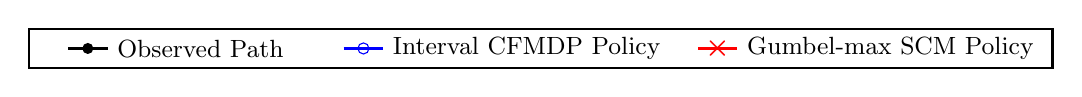
\begin{tikzpicture}[scale=1.0, every node/.style={scale=1.0}]
            \draw[thick, black] (-3, -0.25) rectangle (10, 0.25);
            %
            \draw[black, line width=1pt] (-2.5, 0.0) -- (-2,0.0);
            \fill[black] (-2.25,0.0) circle (2pt); %
            \node[right] at (-2,0.0) {\small Observed Path};
            
            %
            \draw[blue, line width=1pt] (1.0,0.0) -- (1.5,0.0);
            \node[draw=blue, circle, minimum size=4pt, inner sep=0pt] at (1.25,0.0) {}; %
            \node[right] at (1.5,0.0) {\small Interval CFMDP Policy};
            
            %
            \draw[red, line width=1pt] (5.5,0) -- (6,0);
            \node[red] at (5.75,0) {$\boldsymbol{\times}$}; %
            \node[right] at (6,0) {\small Gumbel-max SCM Policy};
        \end{tikzpicture}
    }\\
    %
    \subfigure[\footnotesize Lowest cumulative reward: Interval CFMDP ($312$), Gumbel-max SCM ($312$)]{%
        \resizebox{0.76\columnwidth}{!}{
             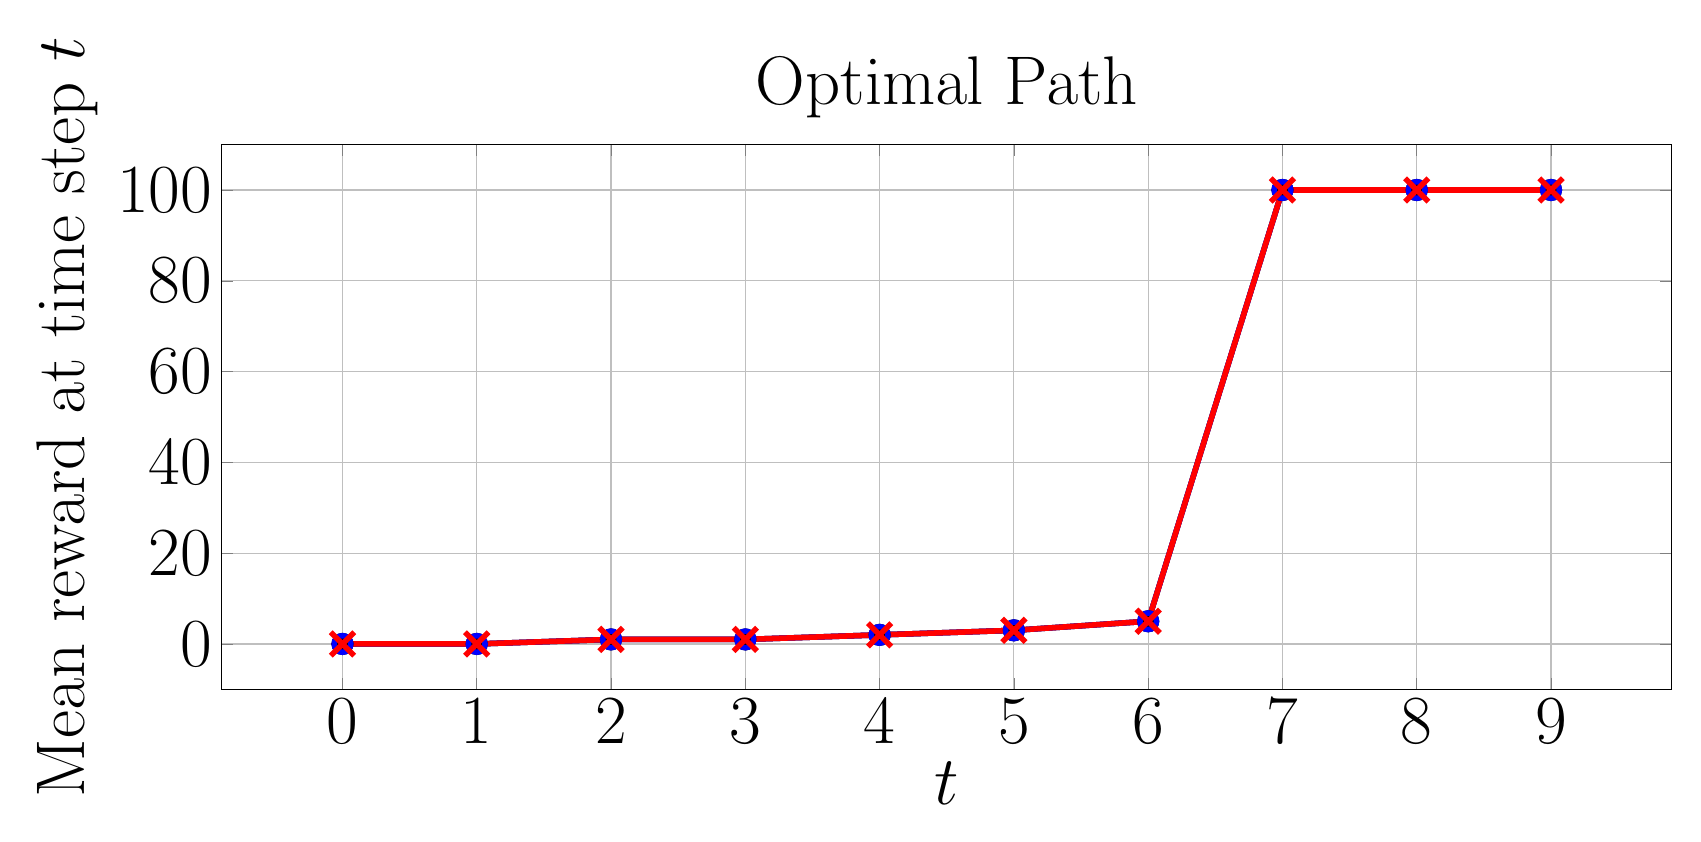
\begin{tikzpicture}
                \begin{axis}[
                    xlabel={$t$},
                    ylabel={Mean reward at time step $t$},
                    title={Optimal Path},
                    grid=both,
                    width=20cm, height=8.5cm,
                    every axis/.style={font=\Huge},
                    %
                ]
                \addplot[
                    color=black, %
                    mark=*, %
                    line width=2pt,
                    mark size=3pt,
                    error bars/.cd,
                    y dir=both, %
                    y explicit, %
                    error bar style={line width=1pt,solid},
                    error mark options={line width=1pt,mark size=4pt,rotate=90}
                ]
                coordinates {
                    (0, 0.0)  +- (0, 0.0)
                    (1, 0.0)  +- (0, 0.0) 
                    (2, 1.0)  +- (0, 0.0) 
                    (3, 1.0)  +- (0, 0.0)
                    (4, 2.0)  +- (0, 0.0)
                    (5, 3.0) +- (0, 0.0)
                    (6, 5.0) +- (0, 0.0)
                    (7, 100.0) +- (0, 0.0)
                    (8, 100.0) +- (0, 0.0)
                    (9, 100.0) +- (0, 0.0)
                };
                %
                \addplot[
                    color=blue, %
                    mark=o, %
                    line width=2pt,
                    mark size=3pt,
                    error bars/.cd,
                    y dir=both, %
                    y explicit, %
                    error bar style={line width=1pt,solid},
                    error mark options={line width=1pt,mark size=4pt,rotate=90}
                ]
                 coordinates {
                    (0, 0.0)  +- (0, 0.0)
                    (1, 0.0)  +- (0, 0.0) 
                    (2, 1.0)  +- (0, 0.0) 
                    (3, 1.0)  +- (0, 0.0)
                    (4, 2.0)  +- (0, 0.0)
                    (5, 3.0) +- (0, 0.0)
                    (6, 5.0) +- (0, 0.0)
                    (7, 100.0) +- (0, 0.0)
                    (8, 100.0) +- (0, 0.0)
                    (9, 100.0) +- (0, 0.0)
                };
                %
                \addplot[
                    color=red, %
                    mark=x, %
                    line width=2pt,
                    mark size=6pt,
                    error bars/.cd,
                    y dir=both, %
                    y explicit, %
                    error bar style={line width=1pt,solid},
                    error mark options={line width=1pt,mark size=4pt,rotate=90}
                ]
                coordinates {
                    (0, 0.0)  +- (0, 0.0)
                    (1, 0.0)  +- (0, 0.0) 
                    (2, 1.0)  +- (0, 0.0) 
                    (3, 1.0)  +- (0, 0.0)
                    (4, 2.0)  +- (0, 0.0)
                    (5, 3.0) +- (0, 0.0)
                    (6, 5.0) +- (0, 0.0)
                    (7, 100.0) +- (0, 0.0)
                    (8, 100.0) +- (0, 0.0)
                    (9, 100.0) +- (0, 0.0)
                };
                \end{axis}
            \end{tikzpicture}
         }
    }
    \hspace{1cm}
    \subfigure[\footnotesize Lowest cumulative reward: Interval CFMDP ($19$), Gumbel-max SCM ($-88$)]{%
         \resizebox{0.76\columnwidth}{!}{
            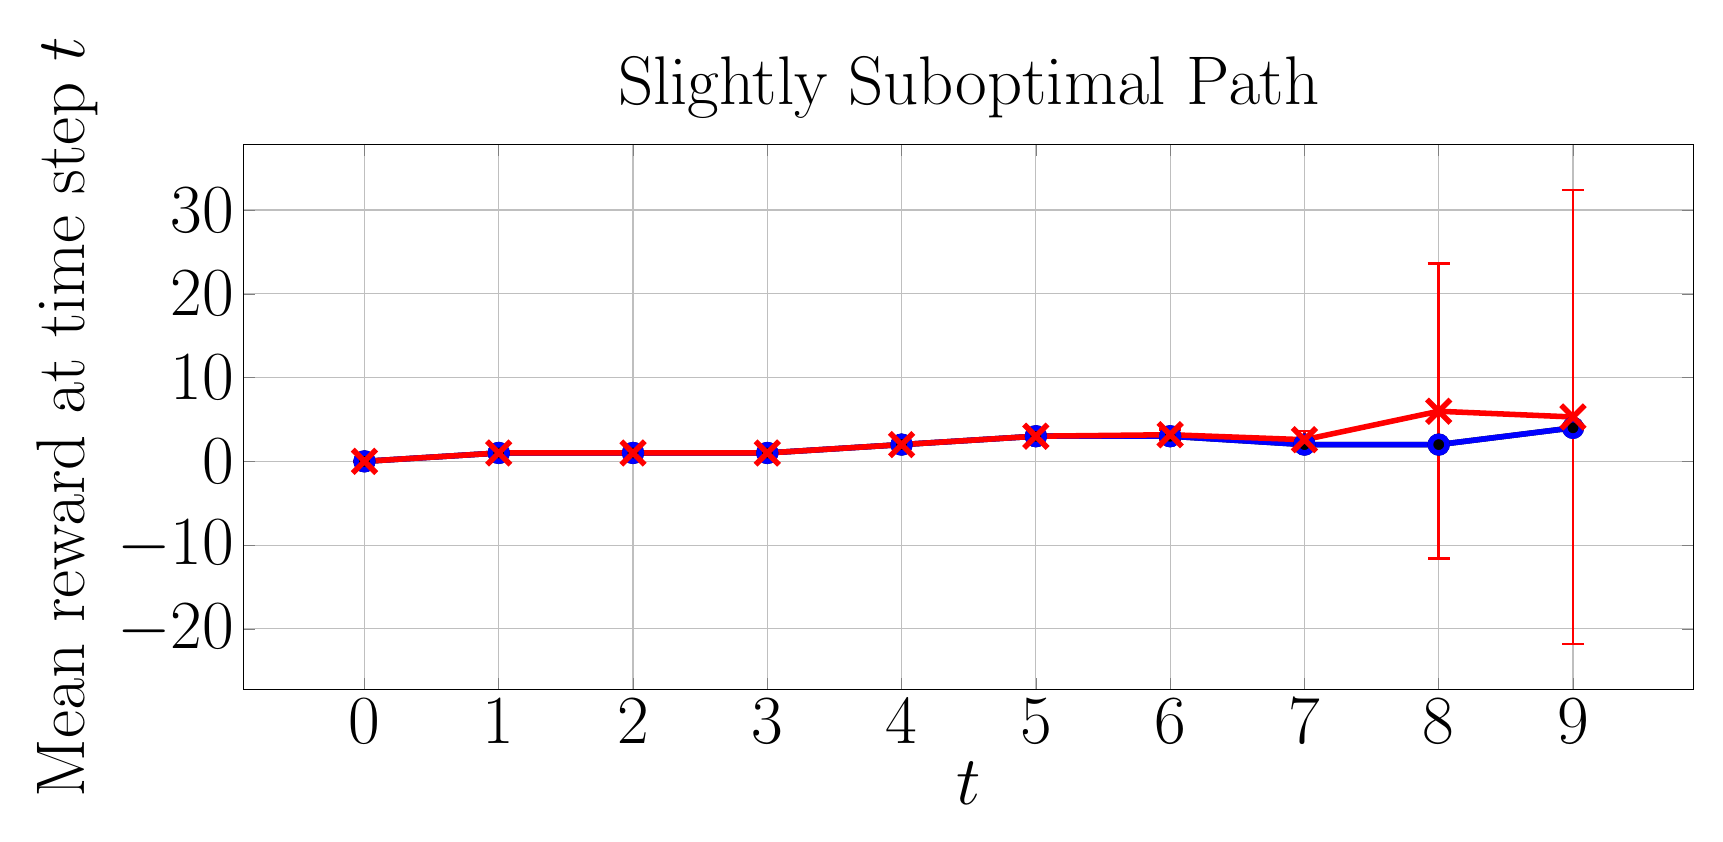
\begin{tikzpicture}
                \begin{axis}[
                    xlabel={$t$},
                    ylabel={Mean reward at time step $t$},
                    title={Slightly Suboptimal Path},
                    grid=both,
                    width=20cm, height=8.5cm,
                    every axis/.style={font=\Huge},
                    %
                ]
                \addplot[
                    color=black, %
                    mark=*, %
                    line width=2pt,
                    mark size=3pt,
                    error bars/.cd,
                    y dir=both, %
                    y explicit, %
                    error bar style={line width=1pt,solid},
                    error mark options={line width=1pt,mark size=4pt,rotate=90}
                ]
              coordinates {
                    (0, 0.0)  +- (0, 0.0)
                    (1, 1.0)  +- (0, 0.0) 
                    (2, 1.0)  +- (0, 0.0) 
                    (3, 1.0)  +- (0, 0.0)
                    (4, 2.0)  +- (0, 0.0)
                    (5, 3.0) +- (0, 0.0)
                    (6, 3.0) +- (0, 0.0)
                    (7, 2.0) +- (0, 0.0)
                    (8, 2.0) +- (0, 0.0)
                    (9, 4.0) +- (0, 0.0)
                };
                %
                \addplot[
                    color=blue, %
                    mark=o, %
                    line width=2pt,
                    mark size=3pt,
                    error bars/.cd,
                    y dir=both, %
                    y explicit, %
                    error bar style={line width=1pt,solid},
                    error mark options={line width=1pt,mark size=4pt,rotate=90}
                ]
              coordinates {
                    (0, 0.0)  +- (0, 0.0)
                    (1, 1.0)  +- (0, 0.0) 
                    (2, 1.0)  +- (0, 0.0) 
                    (3, 1.0)  +- (0, 0.0)
                    (4, 2.0)  +- (0, 0.0)
                    (5, 3.0) +- (0, 0.0)
                    (6, 3.0) +- (0, 0.0)
                    (7, 2.0) +- (0, 0.0)
                    (8, 2.0) +- (0, 0.0)
                    (9, 4.0) +- (0, 0.0)
                };
                %
                \addplot[
                    color=red, %
                    mark=x, %
                    line width=2pt,
                    mark size=6pt,
                    error bars/.cd,
                    y dir=both, %
                    y explicit, %
                    error bar style={line width=1pt,solid},
                    error mark options={line width=1pt,mark size=4pt,rotate=90}
                ]
                coordinates {
                    (0, 0.0)  +- (0, 0.0)
                    (1, 1.0)  +- (0, 0.0) 
                    (2, 1.0)  +- (0, 0.0) 
                    (3, 1.0)  +- (0, 0.0)
                    (4, 2.0)  += (0, 0.0)
                    (5, 3.0)  += (0, 0.0)
                    (6, 3.17847) += (0, 0.62606746) -= (0, 0.62606746)
                    (7, 2.5832885) += (0, 1.04598233) -= (0, 1.04598233)
                    (8, 5.978909) += (0, 17.60137623) -= (0, 17.60137623)
                    (9, 5.297059) += (0, 27.09227512) -= (0, 27.09227512)
                };
                \end{axis}
            \end{tikzpicture}
         }
    }\\[-1.5pt]
    \subfigure[\footnotesize Lowest cumulative reward: Interval CFMDP ($14$), Gumbel-max SCM ($-598$)]{%
         \resizebox{0.76\columnwidth}{!}{
             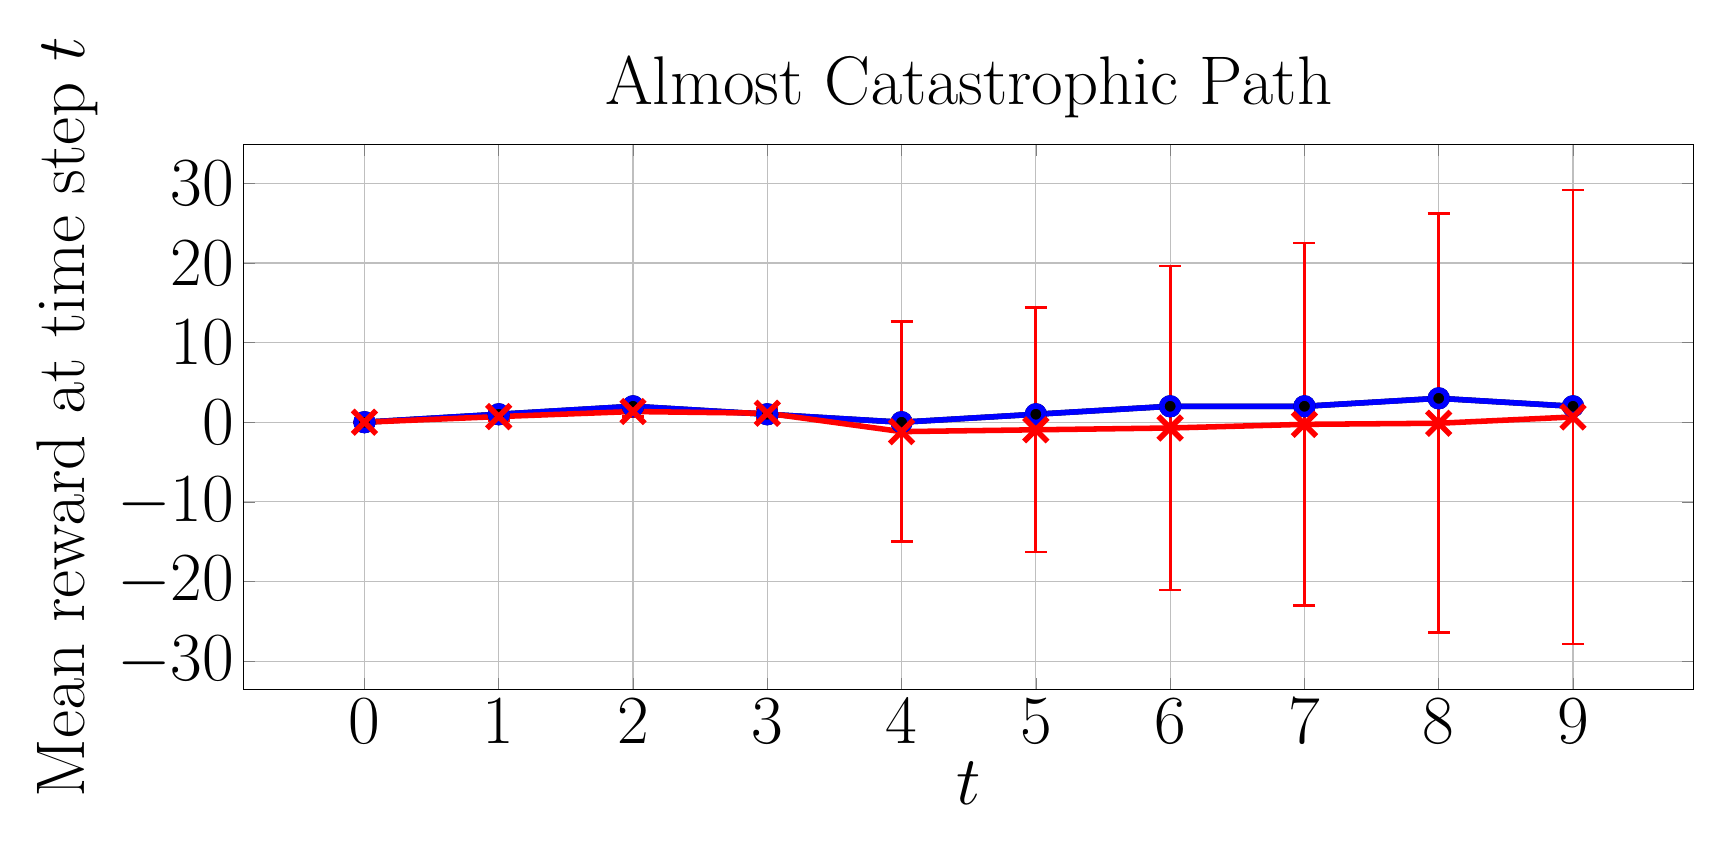
\begin{tikzpicture}
                \begin{axis}[
                    xlabel={$t$},
                    ylabel={Mean reward at time step $t$},
                    title={Almost Catastrophic Path},
                    grid=both,
                    width=20cm, height=8.5cm,
                    every axis/.style={font=\Huge},
                    %
                ]
                \addplot[
                    color=black, %
                    mark=*, %
                    line width=2pt,
                    mark size=3pt,
                    error bars/.cd,
                    y dir=both, %
                    y explicit, %
                    error bar style={line width=1pt,solid},
                    error mark options={line width=1pt,mark size=4pt,rotate=90}
                ]
                coordinates {
                    (0, 0.0)  +- (0, 0.0)
                    (1, 1.0)  +- (0, 0.0) 
                    (2, 2.0)  +- (0, 0.0) 
                    (3, 1.0)  +- (0, 0.0)
                    (4, 0.0)  +- (0, 0.0)
                    (5, 1.0) +- (0, 0.0)
                    (6, 2.0) +- (0, 0.0)
                    (7, 2.0) +- (0, 0.0)
                    (8, 3.0) +- (0, 0.0)
                    (9, 2.0) +- (0, 0.0)
                };
                %
                \addplot[
                    color=blue, %
                    mark=o, %
                    line width=2pt,
                    mark size=3pt,
                    error bars/.cd,
                    y dir=both, %
                    y explicit, %
                    error bar style={line width=1pt,solid},
                    error mark options={line width=1pt,mark size=4pt,rotate=90}
                ]
                coordinates {
                    (0, 0.0)  +- (0, 0.0)
                    (1, 1.0)  +- (0, 0.0) 
                    (2, 2.0)  +- (0, 0.0) 
                    (3, 1.0)  +- (0, 0.0)
                    (4, 0.0)  +- (0, 0.0)
                    (5, 1.0) +- (0, 0.0)
                    (6, 2.0) +- (0, 0.0)
                    (7, 2.0) +- (0, 0.0)
                    (8, 3.0) +- (0, 0.0)
                    (9, 2.0) +- (0, 0.0)
                };
                %
                \addplot[
                    color=red, %
                    mark=x, %
                    line width=2pt,
                    mark size=6pt,
                    error bars/.cd,
                    y dir=both, %
                    y explicit, %
                    error bar style={line width=1pt,solid},
                    error mark options={line width=1pt,mark size=4pt,rotate=90}
                ]
                coordinates {
                    (0, 0.0)  +- (0, 0.0)
                    (1, 0.7065655)  +- (0, 0.4553358) 
                    (2, 1.341673)  +- (0, 0.67091621) 
                    (3, 1.122926)  +- (0, 0.61281824)
                    (4, -1.1821935)  +- (0, 13.82444042)
                    (5, -0.952399)  +- (0, 15.35195457)
                    (6, -0.72672) +- (0, 20.33508414)
                    (7, -0.268983) +- (0, 22.77861454)
                    (8, -0.1310835) +- (0, 26.31013314)
                    (9, 0.65806) +- (0, 28.50670214)
                };
                %
            %
            %
            %
            %
            %
            %
            %
            %
            %
            %
            %
            %
            %
            %
            %
            %
            %
            %
                \end{axis}
            \end{tikzpicture}
         }
    }
    \hspace{1cm}
    \subfigure[\footnotesize Lowest cumulative reward: Interval CFMDP ($-698$), Gumbel-max SCM ($-698$)]{%
         \resizebox{0.76\columnwidth}{!}{
            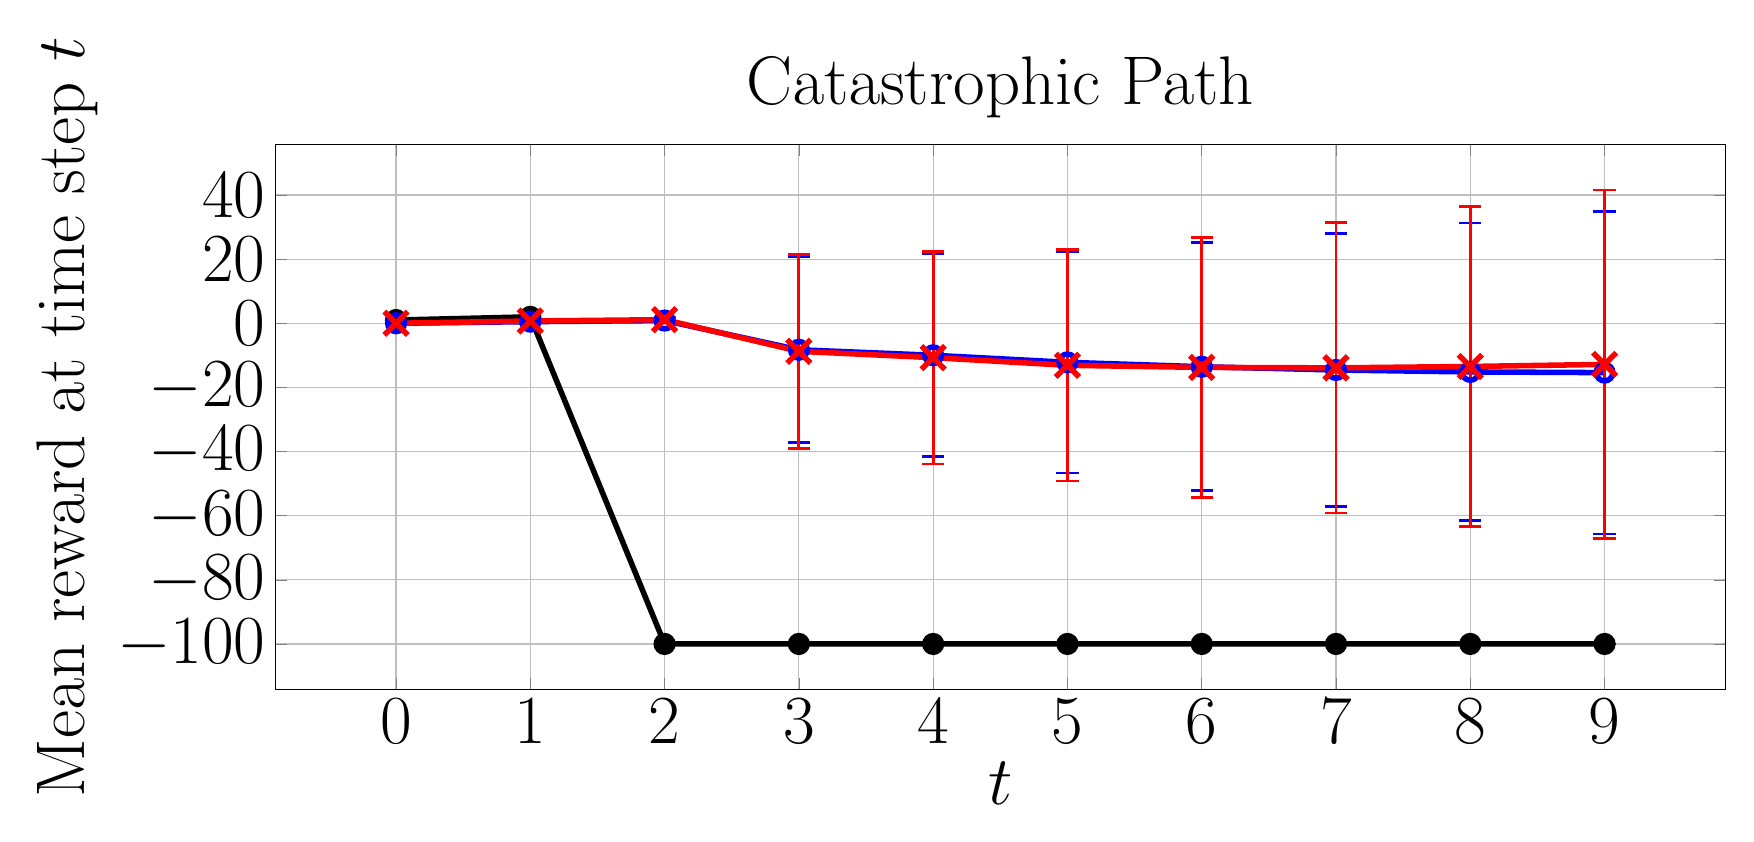
\begin{tikzpicture}
                \begin{axis}[
                    xlabel={$t$},
                    ylabel={Mean reward at time step $t$},
                    title={Catastrophic Path},
                    grid=both,
                    width=20cm, height=8.5cm,
                    every axis/.style={font=\Huge},
                    %
                ]
                \addplot[
                    color=black, %
                    mark=*, %
                    line width=2pt,
                    mark size=3pt,
                    error bars/.cd,
                    y dir=both, %
                    y explicit, %
                    error bar style={line width=1pt,solid},
                    error mark options={line width=1pt,mark size=4pt,rotate=90}
                ]
                coordinates {
                    (0, 1.0)  +- (0, 0.0)
                    (1, 2.0)  +- (0, 0.0) 
                    (2, -100.0)  +- (0, 0.0) 
                    (3, -100.0)  +- (0, 0.0)
                    (4, -100.0)  +- (0, 0.0)
                    (5, -100.0) +- (0, 0.0)
                    (6, -100.0) +- (0, 0.0)
                    (7, -100.0) +- (0, 0.0)
                    (8, -100.0) +- (0, 0.0)
                    (9, -100.0) +- (0, 0.0)
                };
                %
                \addplot[
                    color=blue, %
                    mark=o, %
                    line width=2pt,
                    mark size=3pt,
                    error bars/.cd,
                    y dir=both, %
                    y explicit, %
                    error bar style={line width=1pt,solid},
                    error mark options={line width=1pt,mark size=4pt,rotate=90}
                ]
                coordinates {
                    (0, 0.0)  +- (0, 0.0)
                    (1, 0.504814)  +- (0, 0.49997682) 
                    (2, 0.8439835)  +- (0, 0.76831917) 
                    (3, -8.2709165)  +- (0, 28.93656754)
                    (4, -9.981082)  +- (0, 31.66825363)
                    (5, -12.1776325) +- (0, 34.53463233)
                    (6, -13.556076) +- (0, 38.62845372)
                    (7, -14.574418) +- (0, 42.49603359)
                    (8, -15.1757075) +- (0, 46.41913968)
                    (9, -15.3900395) +- (0, 50.33563368)
                };
                %
                \addplot[
                    color=red, %
                    mark=x, %
                    line width=2pt,
                    mark size=6pt,
                    error bars/.cd,
                    y dir=both, %
                    y explicit, %
                    error bar style={line width=1pt,solid},
                    error mark options={line width=1pt,mark size=4pt,rotate=90}
                ]
                coordinates {
                    (0, 0.0)  +- (0, 0.0)
                    (1, 0.701873)  +- (0, 0.45743556) 
                    (2, 1.1227805)  +- (0, 0.73433129) 
                    (3, -8.7503255)  +- (0, 30.30257976)
                    (4, -10.722092)  +- (0, 33.17618589)
                    (5, -13.10721)  +- (0, 36.0648089)
                    (6, -13.7631645) +- (0, 40.56553451)
                    (7, -13.909043) +- (0, 45.23829402)
                    (8, -13.472517) +- (0, 49.96270296)
                    (9, -12.8278835) +- (0, 54.38618735)
                };
                %
            %
            %
            %
            %
            %
            %
            %
            %
            %
            %
            %
            %
            %
            %
            %
            %
            %
            %
                \end{axis}
            \end{tikzpicture}
         }
    }
    \caption{Average instant reward of CF paths induced by policies on GridWorld $p=0.4$.}
    \label{fig: reward p=0.4}
\end{figure*}

\subsection{Experimental Setup}
To compare policy performance, we measure the average rewards of counterfactual paths induced by our policy and the Gumbel-max policy by uniformly sampling $200$ counterfactual MDPs from the ICFMDP and generating $10,000$ counterfactual paths over each sampled CFMDP. \jl{Since the interval CFMDP depends on the observed path, we select $4$  paths of varying optimality to evaluate how the observed path impacts the performance of both policies: an optimal path, a slightly suboptimal path that could reach the optimal reward with a few changes, a catastrophic path that enters a catastrophic, terminal state with low reward, and an almost catastrophic path that was close to entering a catastrophic state.} When measuring the average probability bound widths and execution time needed to generate the ICFMDPs, we averaged over $20$ randomly generated observed paths
\footnote{Further training details are provided in Appendix \ref{app: training details}, and the code is provided at \href{https://github.com/ddv-lab/robust-cf-inference-in-MDPs}{https://github.com/ddv-lab/robust-cf-inference-in-MDPs}
%
%
.}.

\subsection{GridWorld}
\jl{The GridWorld MDP is a $4 \times 4$ grid where an agent must navigate from the top-left corner to the goal state in the bottom-right corner, avoiding a dangerous terminal state in the centre. At each time step, the agent can move up, down, left, or right, but there is a small probability (controlled by hyper-parameter $p$) of moving in an unintended direction. As the agent nears the goal, the reward for each state increases, culminating in a reward of $+100$ for reaching the goal. Entering the dangerous state results in a penalty of $-100$. We use two versions of GridWorld: a less stochastic version with $p=0.9$ (i.e., $90$\% chance of moving in the chosen direction) and a more stochastic version with $p=0.4$.}

\paragraph{GridWorld ($p=0.9$)}
When $p=0.9$, the counterfactual probability bounds are typically narrow (see Table \ref{tab:nonzero_probs} for average measurements). Consequently, as shown in Figure \ref{fig: reward p=0.9}, both policies are nearly identical and perform similarly well across the optimal, slightly suboptimal, and catastrophic paths.
%
However, for the almost catastrophic path, the interval CFMDP path is more conservative and follows the observed path more closely (as this is where the probability bounds are narrowest), which typically requires one additional step to reach the goal state than the Gumbel-max SCM policy.
%

\paragraph{GridWorld ($p=0.4$)}
\jl{When $p=0.4$, the GridWorld environment becomes more uncertain, increasing the risk of entering the dangerous state even if correct actions are chosen. Thus, as shown in Figure \ref{fig: reward p=0.4}, the interval CFMDP policy adopts a more conservative approach, avoiding deviation from the observed policy if it cannot guarantee higher counterfactual rewards (see the slightly suboptimal and almost catastrophic paths), whereas the Gumbel-max SCM is inconsistent: it can yield higher rewards, but also much lower rewards, reflected in the wide error bars.} For the catastrophic path, both policies must deviate from the observed path to achieve a higher reward and, in this case, perform similarly.
%
%
%
%
\subsection{Sepsis}
The Sepsis MDP \citep{oberst2019counterfactual} simulates trajectories of Sepsis patients. Each state consists of four vital signs (heart rate, blood pressure, oxygen concentration, and glucose levels), categorised as low, normal, or high.
and three treatments that can be toggled on/off at each time step (8 actions in total). Unlike \citet{oberst2019counterfactual}, we scale rewards based on the number of out-of-range vital signs, between $-1000$ (patient dies) and $1000$ (patient discharged). \jl{Like the GridWorld $p=0.4$ experiment, the Sepsis MDP is highly uncertain, as many states are equally likely to lead to optimal and poor outcomes. Thus, as shown in Figure \ref{fig: reward sepsis}, both policies follow the observed optimal and almost catastrophic paths to guarantee rewards are no worse than the observation.} However, improving the catastrophic path requires deviating from the observation. Here, the Gumbel-max SCM policy, on average, performs better than the interval CFMDP policy. But, since both policies have lower bounds clipped at $-1000$, neither policy reliably improves over the observation. In contrast, for the slightly suboptimal path, the interval CFMDP policy performs significantly better, shown by its higher lower bounds. 
Moreover, in these two cases, the worst-case counterfactual path generated by the interval CFMDP policy is better than that of the Gumbel-max SCM policy,
indicating its greater robustness.
%
\begin{figure*}
    \centering
     \resizebox{0.6\textwidth}{!}{
        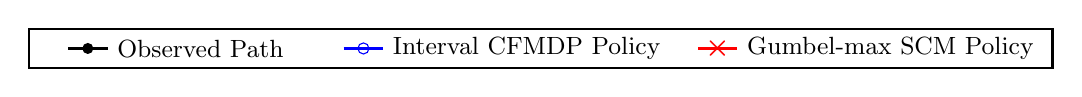
\begin{tikzpicture}[scale=1.0, every node/.style={scale=1.0}]
            \draw[thick, black] (-3, -0.25) rectangle (10, 0.25);
            %
            \draw[black, line width=1pt] (-2.5, 0.0) -- (-2,0.0);
            \fill[black] (-2.25,0.0) circle (2pt); %
            \node[right] at (-2,0.0) {\small Observed Path};
            
            %
            \draw[blue, line width=1pt] (1.0,0.0) -- (1.5,0.0);
            \node[draw=blue, circle, minimum size=4pt, inner sep=0pt] at (1.25,0.0) {}; %
            \node[right] at (1.5,0.0) {\small Interval CFMDP Policy};
            
            %
            \draw[red, line width=1pt] (5.5,0) -- (6,0);
            \node[red] at (5.75,0) {$\boldsymbol{\times}$}; %
            \node[right] at (6,0) {\small Gumbel-max SCM Policy};
        \end{tikzpicture}
    }\\
    \subfigure[\footnotesize Lowest cumulative reward: Interval CFMDP ($8000$), Gumbel-max SCM ($8000$)]{%
         \resizebox{0.76\columnwidth}{!}{
             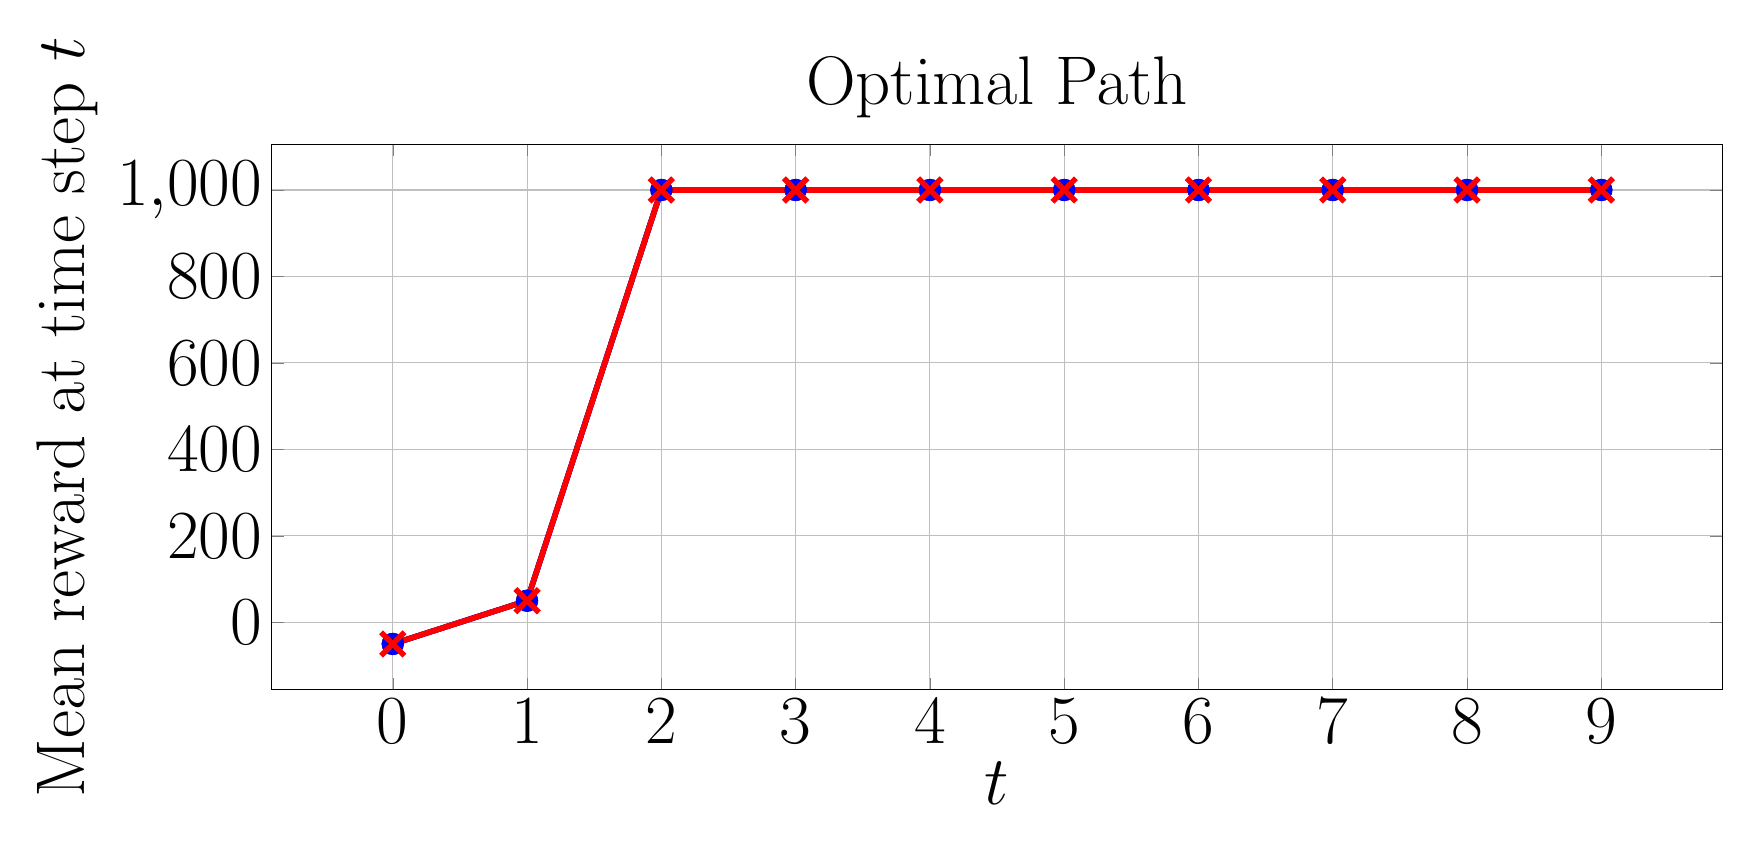
\begin{tikzpicture}
                \begin{axis}[
                    xlabel={$t$},
                    ylabel={Mean reward at time step $t$},
                    title={Optimal Path},
                    grid=both,
                    width=20cm, height=8.5cm,
                    every axis/.style={font=\Huge},
                    %
                ]
                \addplot[
                    color=black, %
                    mark=*, %
                    line width=2pt,
                    mark size=3pt,
                ]
                coordinates {
                    (0, -50.0)
                    (1, 50.0)
                    (2, 1000.0)
                    (3, 1000.0)
                    (4, 1000.0)
                    (5, 1000.0)
                    (6, 1000.0)
                    (7, 1000.0)
                    (8, 1000.0)
                    (9, 1000.0)
                };
                %
                \addplot[
                    color=blue, %
                    mark=o, %
                    line width=2pt,
                    mark size=3pt,
                    error bars/.cd,
                    y dir=both, %
                    y explicit, %
                    error bar style={line width=1pt,solid},
                    error mark options={line width=1pt,mark size=4pt,rotate=90}
                ]
                coordinates {
                    (0, -50.0)  +- (0, 0.0)
                    (1, 50.0)  +- (0, 0.0) 
                    (2, 1000.0)  +- (0, 0.0) 
                    (3, 1000.0)  +- (0, 0.0)
                    (4, 1000.0)  +- (0, 0.0)
                    (5, 1000.0) +- (0, 0.0)
                    (6, 1000.0) +- (0, 0.0)
                    (7, 1000.0) +- (0, 0.0)
                    (8, 1000.0) +- (0, 0.0)
                    (9, 1000.0) +- (0, 0.0)
                };
                %
                \addplot[
                    color=red, %
                    mark=x, %
                    line width=2pt,
                    mark size=6pt,
                    error bars/.cd,
                    y dir=both, %
                    y explicit, %
                    error bar style={line width=1pt,solid},
                    error mark options={line width=1pt,mark size=4pt,rotate=90}
                ]
                coordinates {
                    (0, -50.0)  +- (0, 0.0)
                    (1, 50.0)  +- (0, 0.0) 
                    (2, 1000.0)  +- (0, 0.0) 
                    (3, 1000.0)  +- (0, 0.0)
                    (4, 1000.0)  +- (0, 0.0)
                    (5, 1000.0) +- (0, 0.0)
                    (6, 1000.0) +- (0, 0.0)
                    (7, 1000.0) +- (0, 0.0)
                    (8, 1000.0) +- (0, 0.0)
                    (9, 1000.0) +- (0, 0.0)
                };
                %
                \end{axis}
            \end{tikzpicture}
         }
    }
    \hspace{1cm}
    \subfigure[\footnotesize Lowest cumulative reward: Interval CFMDP ($-5980$), Gumbel-max SCM ($-8000$)]{%
         \resizebox{0.76\columnwidth}{!}{
            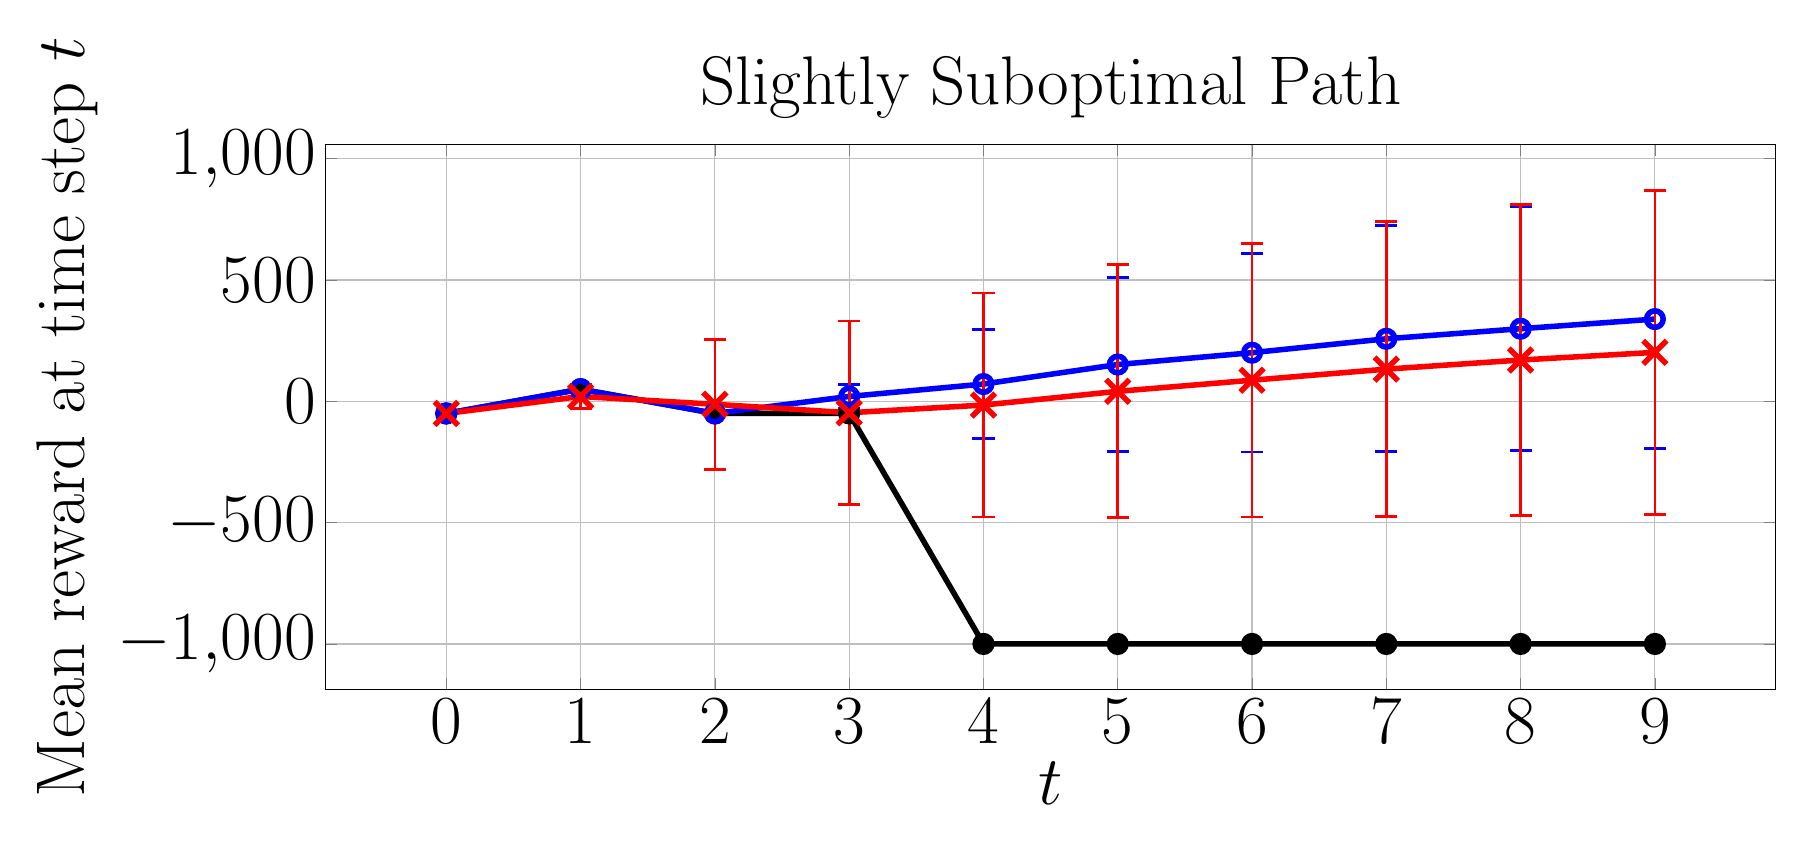
\begin{tikzpicture}
                \begin{axis}[
                    xlabel={$t$},
                    ylabel={Mean reward at time step $t$},
                    title={Slightly Suboptimal Path},
                    grid=both,
                    width=20cm, height=8.5cm,
                    every axis/.style={font=\Huge},
                    %
                ]
               \addplot[
                    color=black, %
                    mark=*, %
                    line width=2pt,
                    mark size=3pt,
                ]
                coordinates {
                    (0, -50.0)
                    (1, 50.0)
                    (2, -50.0)
                    (3, -50.0)
                    (4, -1000.0)
                    (5, -1000.0)
                    (6, -1000.0)
                    (7, -1000.0)
                    (8, -1000.0)
                    (9, -1000.0)
                };
                %
                \addplot[
                    color=blue, %
                    mark=o, %
                    line width=2pt,
                    mark size=3pt,
                    error bars/.cd,
                    y dir=both, %
                    y explicit, %
                    error bar style={line width=1pt,solid},
                    error mark options={line width=1pt,mark size=4pt,rotate=90}
                ]
                coordinates {
                    (0, -50.0)  +- (0, 0.0)
                    (1, 50.0)  +- (0, 0.0) 
                    (2, -50.0)  +- (0, 0.0) 
                    (3, 20.0631)  +- (0, 49.97539413)
                    (4, 71.206585)  +- (0, 226.02033693)
                    (5, 151.60797) +- (0, 359.23292559)
                    (6, 200.40593) +- (0, 408.86185176)
                    (7, 257.77948) +- (0, 466.10372804)
                    (8, 299.237465) +- (0, 501.82579506)
                    (9, 338.9129) +- (0, 532.06124996)
                };
                %
                \addplot[
                    color=red, %
                    mark=x, %
                    line width=2pt,
                    mark size=6pt,
                    error bars/.cd,
                    y dir=both, %
                    y explicit, %
                    error bar style={line width=1pt,solid},
                    error mark options={line width=1pt,mark size=4pt,rotate=90}
                ]
                coordinates {
                    (0, -50.0)  +- (0, 0.0)
                    (1, 20.00736)  +- (0, 49.99786741) 
                    (2, -12.282865)  +- (0, 267.598755) 
                    (3, -47.125995)  +- (0, 378.41755832)
                    (4, -15.381965)  +- (0, 461.77616558)
                    (5, 41.15459) +- (0, 521.53189262)
                    (6, 87.01595) +- (0, 564.22243126 )
                    (7, 132.62376) +- (0, 607.31338037)
                    (8, 170.168145) +- (0, 641.48013693)
                    (9, 201.813135) +- (0, 667.29441777)
                };
                %
                %
                %
                %
                %
                %
                %
                %
                %
                %
                %
                %
                %
                %
                %
                %
                %
                %
                %
                \end{axis}
            \end{tikzpicture}
         }
    }\\[-1.5pt]
    \subfigure[\footnotesize Lowest cumulative reward: Interval CFMDP ($100$), Gumbel-max SCM ($100$)]{%
         \resizebox{0.76\columnwidth}{!}{
             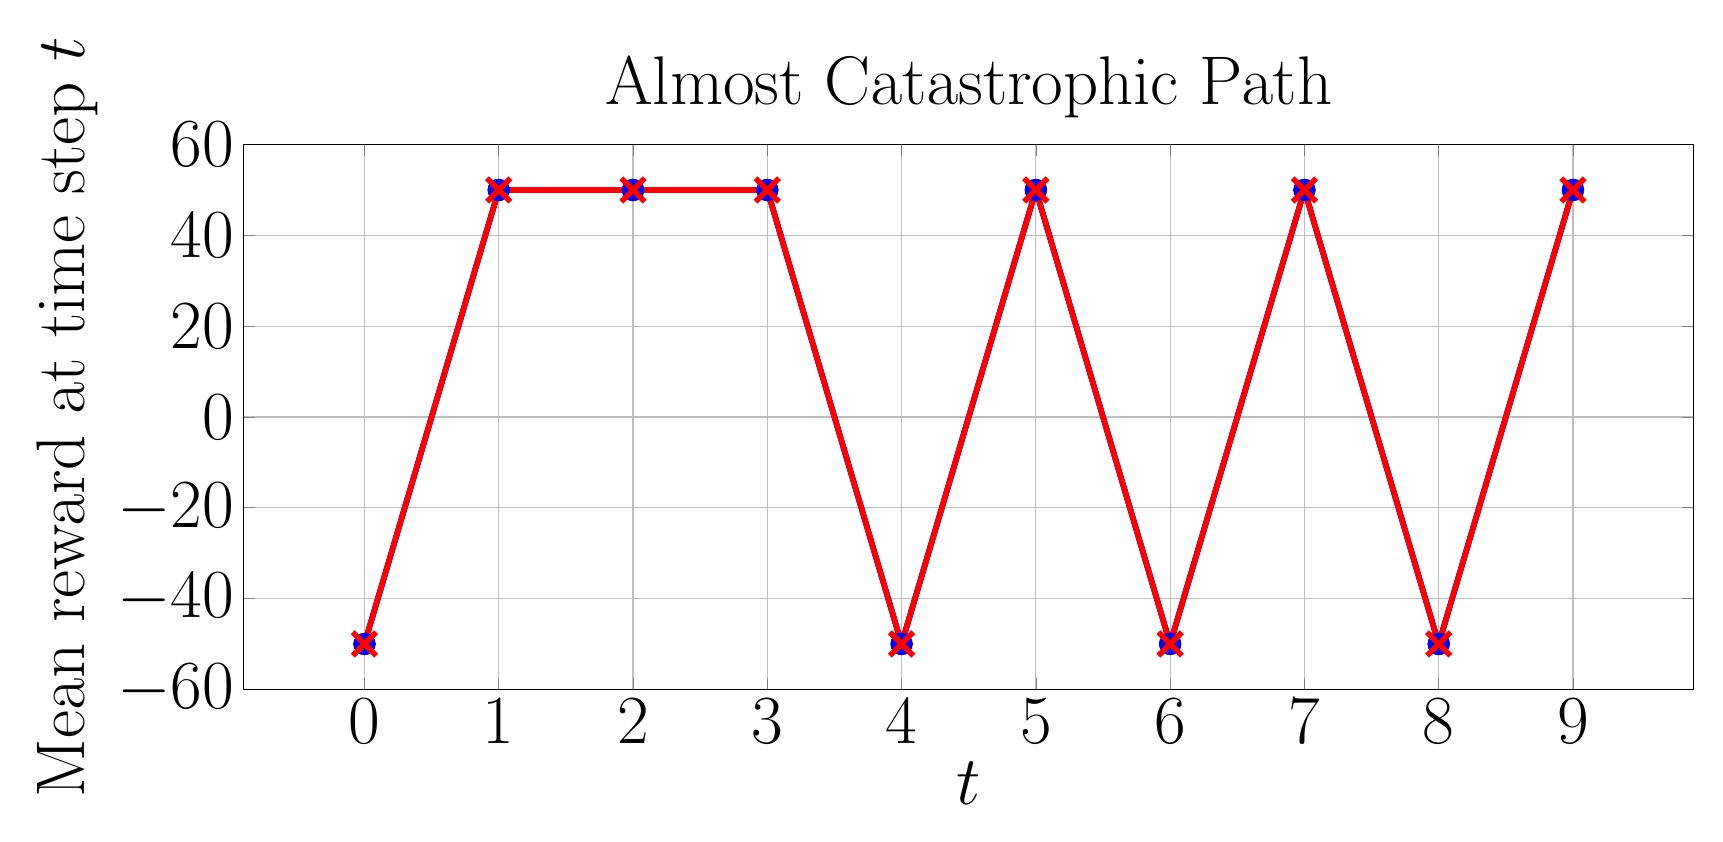
\begin{tikzpicture}
                \begin{axis}[
                    xlabel={$t$},
                    ylabel={Mean reward at time step $t$},
                    title={Almost Catastrophic Path},
                    grid=both,
                    every axis/.style={font=\Huge},
                    width=20cm, height=8.5cm,
                    %
                ]
               \addplot[
                    color=black, %
                    mark=*, %
                    line width=2pt,
                    mark size=3pt,
                ]
                coordinates {
                    (0, -50.0)
                    (1, 50.0)
                    (2, 50.0)
                    (3, 50.0)
                    (4, -50.0)
                    (5, 50.0)
                    (6, -50.0)
                    (7, 50.0)
                    (8, -50.0)
                    (9, 50.0)
                };
                %
                %
                \addplot[
                    color=blue, %
                    mark=o, %
                    line width=2pt,
                    mark size=3pt,
                    error bars/.cd,
                    y dir=both, %
                    y explicit, %
                    error bar style={line width=1pt,solid},
                    error mark options={line width=1pt,mark size=4pt,rotate=90}
                ]
                coordinates {
                    (0, -50.0)  +- (0, 0.0)
                    (1, 50.0)  +- (0, 0.0) 
                    (2, 50.0)  +- (0, 0.0) 
                    (3, 50.0)  +- (0, 0.0)
                    (4, -50.0)  +- (0, 0.0)
                    (5, 50.0) +- (0, 0.0)
                    (6, -50.0) +- (0, 0.0)
                    (7, 50.0) +- (0, 0.0)
                    (8, -50.0) +- (0, 0.0)
                    (9, 50.0) +- (0, 0.0)
                };
                %
                \addplot[
                    color=red, %
                    mark=x, %
                    line width=2pt,
                    mark size=6pt,
                    error bars/.cd,
                    y dir=both, %
                    y explicit, %
                    error bar style={line width=1pt,solid},
                    error mark options={line width=1pt,mark size=4pt,rotate=90}
                ]
                coordinates {
                    (0, -50.0)  +- (0, 0.0)
                    (1, 50.0)  +- (0, 0.0) 
                    (2, 50.0)  +- (0, 0.0) 
                    (3, 50.0)  +- (0, 0.0)
                    (4, -50.0)  +- (0, 0.0)
                    (5, 50.0) +- (0, 0.0)
                    (6, -50.0) +- (0, 0.0)
                    (7, 50.0) +- (0, 0.0)
                    (8, -50.0) +- (0, 0.0)
                    (9, 50.0) +- (0, 0.0)
                };
                %
                %
                %
                %
                %
                %
                %
                %
                %
                %
                %
                %
                %
                %
                %
                %
                %
                %
                %
                \end{axis}
            \end{tikzpicture}
         }
    }
    \hspace{1cm}
    \subfigure[\footnotesize Lowest cumulative reward: Interval CFMDP ($-7150$), Gumbel-max SCM ($-9050$)]{%
         \resizebox{0.76\columnwidth}{!}{
            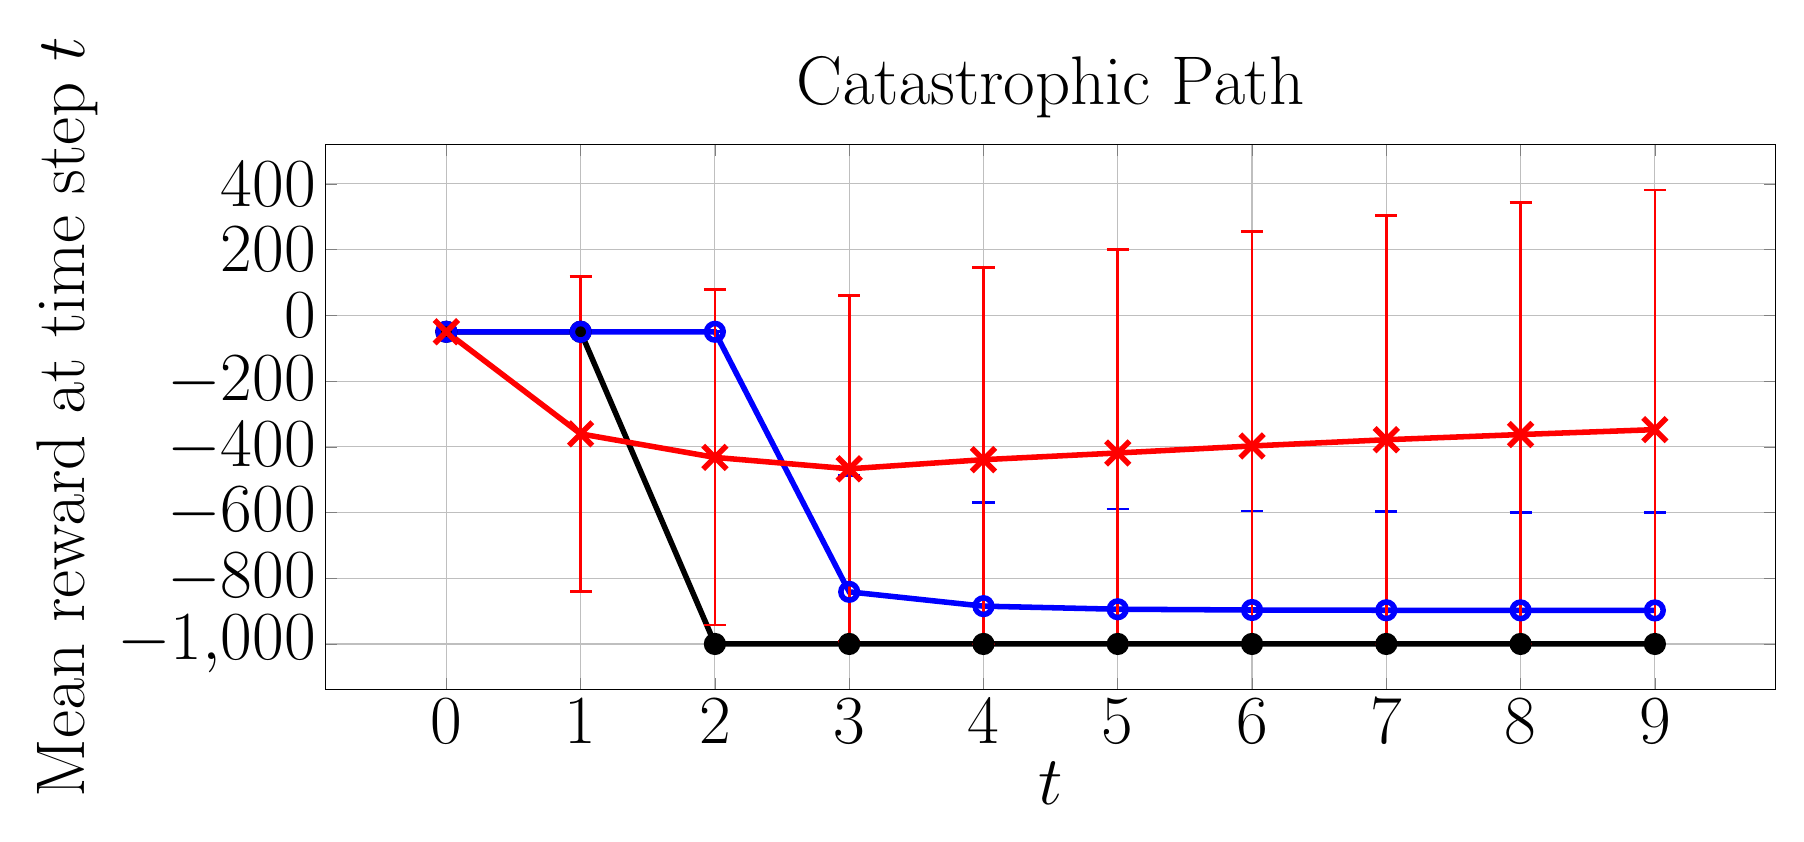
\begin{tikzpicture}
                \begin{axis}[
                    xlabel={$t$},
                    ylabel={Mean reward at time step $t$},
                    title={Catastrophic Path},
                    grid=both,
                    width=20cm, height=8.5cm,
                    every axis/.style={font=\Huge},
                    %
                ]
               \addplot[
                    color=black, %
                    mark=*, %
                    line width=2pt,
                    mark size=3pt,
                ]
                coordinates {
                    (0, -50.0)
                    (1, -50.0)
                    (2, -1000.0)
                    (3, -1000.0)
                    (4, -1000.0)
                    (5, -1000.0)
                    (6, -1000.0)
                    (7, -1000.0)
                    (8, -1000.0)
                    (9, -1000.0)
                };
                %
                %
                \addplot[
                    color=blue, %
                    mark=o, %
                    line width=2pt,
                    mark size=3pt,
                    error bars/.cd,
                    y dir=both, %
                    y explicit, %
                    error bar style={line width=1pt,solid},
                    error mark options={line width=1pt,mark size=4pt,rotate=90}
                ]
                coordinates {
                    (0, -50.0)  +- (0, 0.0)
                    (1, -50.0)  +- (0, 0.0) 
                    (2, -50.0)  +- (0, 0.0) 
                    (3, -841.440725)  += (0, 354.24605512) -= (0, 158.559275)
                    (4, -884.98225)  += (0, 315.37519669) -= (0, 115.01775)
                    (5, -894.330425) += (0, 304.88572805) -= (0, 105.669575)
                    (6, -896.696175) += (0, 301.19954514) -= (0, 103.303825)
                    (7, -897.4635) += (0, 299.61791279) -= (0, 102.5365)
                    (8, -897.77595) += (0, 298.80392585) -= (0, 102.22405)
                    (9, -897.942975) += (0, 298.32920557) -= (0, 102.057025)
                };
                %
                \addplot[
                    color=red, %
                    mark=x, %
                    line width=2pt,
                    mark size=6pt,
                    error bars/.cd,
                    y dir=both, %
                    y explicit, %
                    error bar style={line width=1pt,solid},
                    error mark options={line width=1pt,mark size=4pt,rotate=90}
                ]
            coordinates {
                    (0, -50.0)  +- (0, 0.0)
                    (1, -360.675265)  +- (0, 479.39812699) 
                    (2, -432.27629)  +- (0, 510.38620897) 
                    (3, -467.029545)  += (0, 526.36009628) -= (0, 526.36009628)
                    (4, -439.17429)  += (0, 583.96638919) -= (0, 560.82571)
                    (5, -418.82704) += (0, 618.43027478) -= (0, 581.17296)
                    (6, -397.464895) += (0, 652.67322574) -= (0, 602.535105)
                    (7, -378.49052) += (0, 682.85407033) -= (0, 621.50948)
                    (8, -362.654195) += (0, 707.01412023) -= (0, 637.345805)
                    (9, -347.737935) += (0, 729.29076479) -= (0, 652.262065)
                };
                %
                %
                %
                %
                %
                %
                %
                %
                %
                %
                %
                %
                %
                %
                %
                %
                %
                %
                %
                \end{axis}
            \end{tikzpicture}
         }
    }
    \caption{Average instant reward of CF paths induced by policies on Sepsis.}
    \label{fig: reward sepsis}
\end{figure*}

%
%
%
\subsection{Interval CFMDP Bounds}
%
%
Table \ref{tab:nonzero_probs} presents the mean counterfactual probability bound widths (excluding transitions where the upper bound is $0$) for each MDP, averaged over 20 observed paths. We compare the bounds under counterfactual stability (CS) and monotonicity (M) assumptions, CS alone, and no assumptions. This shows that the assumptions marginally reduce the bound widths, indicating the assumptions tighten the bounds without excluding too many causal models, as intended.
\renewcommand{\arraystretch}{1}

\begin{table}
\centering
\caption{Mean width of counterfactual probability bounds}
\resizebox{0.8\columnwidth}{!}{%
\begin{tabular}{|c|c|c|c|}
\hline
\multirow{2}{*}{\textbf{Environment}} & \multicolumn{3}{c|}{\textbf{Assumptions}} \\ \cline{2-4}
 & \textbf{CS + M} & \textbf{CS} & \textbf{None\tablefootnote{\jl{Equivalent to \citet{li2024probabilities}'s bounds (see Section \ref{sec: equivalence with Li}).}}} \\ \hline
\textbf{GridWorld} ($p=0.9$) & 0.0817 & 0.0977 & 0.100 \\ \hline
\textbf{GridWorld} ($p=0.4$) & 0.552  & 0.638  & 0.646 \\ \hline
\textbf{Sepsis} & 0.138 & 0.140 & 0.140 \\ \hline
\end{tabular}
}
\label{tab:nonzero_probs}
\end{table}


\subsection{Execution Times}
Table \ref{tab: times} compares the average time needed to generate the interval CFMDP vs.\ the Gumbel-max SCM CFMDP for 20 observations.
The GridWorld algorithms were run single-threaded, while the Sepsis experiments were run in parallel.
Generating the interval CFMDP is significantly faster as it uses exact analytical bounds, whereas the Gumbel-max CFMDP requires sampling from the Gumbel distribution to estimate counterfactual transition probabilities. \jl{Since constructing the counterfactual MDP models is the main bottleneck in both approaches, ours is more efficient overall and suitable for larger MDPs.}
\begin{table}
\centering
\caption{Mean execution time to generate CFMDPs}
\resizebox{0.99\columnwidth}{!}{%
\begin{tabular}{|c|c|c|}
\hline
\multirow{2}{*}{\textbf{Environment}} & \multicolumn{2}{c|}{\textbf{Mean Execution Time (s)}} \\ \cline{2-3} 
                                      & \textbf{Interval CFMDP} & \textbf{Gumbel-max CFMDP} \\ \hline
\textbf{GridWorld ($p=0.9$) }                  & 0.261                   & 56.1                      \\ \hline
\textbf{GridWorld ($p=0.4$)  }                 & 0.336                   & 54.5                      \\ \hline
\textbf{Sepsis}                                 & 688                     & 2940                      \\ \hline
\end{tabular}%
}
\label{tab: times}
\end{table}

\section{Related Works}
\subsection{Claim Verification}

Early approaches to claim verification focused on fine-tuning pre-trained models, either by concatenating evidence and claims into a single input~\cite{aly2021feverous, thorne2018fever, hu2022dual} or processing evidence separately and aggregating the results~\cite{soleimani2020bert, jiang2021exploring,gi-etal-2021-verdict}. Graph Neural Networks have also been applied to capture relationships between evidence pieces~\cite{gong2024heterogeneous, Zhaotransxh, Chenevidencenet}. With the impressive generative capabilities demonstrated by large language models (LLMs), many studies have turned to LLMs for claim verification~\cite{ma-etal-2024-ex}. FACT-GPT~\cite{factgpt} and FactLlama~\cite{cheung2023factllama} fine-tune LLMs to directly predict the truthfulness of claims. Factscore~\cite{min2023factscore} employs systematic decomposition to assess the factuality of individual claim segments, while ProgramFC~\cite{pan2023fact} frames claim verification as step-wise program execution. Other works, such as \citet{li2023self}, \citet{chen2022generating}, and \citet{rani2023factify}, transform the verification task into a series of sub-questions to be answered.


\subsection{Chain of Thought Reasoning (CoT)}
Chain of Thought (CoT) reasoning~\cite{wei2022chain} was proposed to help LLMs solve complex problems by breaking them down into intermediate step-by-step reasoning. \citet{kojima2022large} demonstrated that adding a prompt such as ``Let's think step by step'' significantly boosts LLM performance. CoT reasoning has been applied to a variety of tasks, including claim verification. Studies like \citet{hu2023large} and \citet{dougrez2024assessing} evaluate CoT methods in different contexts. FOLK~\cite{wang2023explainable} leverages LLMs to transform claims into first-order logic as intermediate steps for explainable verification.

\subsection{Self-Improvement Methods}
Self-improvement methods for LLMs have garnered attention in recent years, where models are fine-tuned on their self-generated solutions, optionally iterating this process~\cite{hosseini2024v}. $\text{ReST}^{EM}$~\cite{singh2023beyond} generates reasoning chains for solving math problems and selects those leading to correct answers for retraining. RFT~\cite{yuan2023scaling} enhances reasoning chain diversity by sampling multiple chains before selection. STaR~\cite{zelikman2022star} introduces hints during reasoning generation for chains that lead to incorrect results. V-STaR~\cite{hosseini2024v} incorporates Direct Preference Optimization~\cite{rafailov2023direct} into the self-improvement process. Our method shares similarities with STaR. We are the first to apply self-improvement to claim verification. We also highlight the unique challenges of claim verification, distinguishing it from tasks like math problem-solving, and address these challenges through the integration of structured reasoning design. 
\section{Conclusion}
In this work, we propose a simple yet effective approach, called SMILE, for graph few-shot learning with fewer tasks. Specifically, we introduce a novel dual-level mixup strategy, including within-task and across-task mixup, for enriching the diversity of nodes within each task and the diversity of tasks. Also, we incorporate the degree-based prior information to learn expressive node embeddings. Theoretically, we prove that SMILE effectively enhances the model's generalization performance. Empirically, we conduct extensive experiments on multiple benchmarks and the results suggest that SMILE significantly outperforms other baselines, including both in-domain and cross-domain few-shot settings.

\clearpage

\bibliographystyle{unsrtnat}
\bibliography{neurips_2024}

\subsection{Lloyd-Max Algorithm}
\label{subsec:Lloyd-Max}
For a given quantization bitwidth $B$ and an operand $\bm{X}$, the Lloyd-Max algorithm finds $2^B$ quantization levels $\{\hat{x}_i\}_{i=1}^{2^B}$ such that quantizing $\bm{X}$ by rounding each scalar in $\bm{X}$ to the nearest quantization level minimizes the quantization MSE. 

The algorithm starts with an initial guess of quantization levels and then iteratively computes quantization thresholds $\{\tau_i\}_{i=1}^{2^B-1}$ and updates quantization levels $\{\hat{x}_i\}_{i=1}^{2^B}$. Specifically, at iteration $n$, thresholds are set to the midpoints of the previous iteration's levels:
\begin{align*}
    \tau_i^{(n)}=\frac{\hat{x}_i^{(n-1)}+\hat{x}_{i+1}^{(n-1)}}2 \text{ for } i=1\ldots 2^B-1
\end{align*}
Subsequently, the quantization levels are re-computed as conditional means of the data regions defined by the new thresholds:
\begin{align*}
    \hat{x}_i^{(n)}=\mathbb{E}\left[ \bm{X} \big| \bm{X}\in [\tau_{i-1}^{(n)},\tau_i^{(n)}] \right] \text{ for } i=1\ldots 2^B
\end{align*}
where to satisfy boundary conditions we have $\tau_0=-\infty$ and $\tau_{2^B}=\infty$. The algorithm iterates the above steps until convergence.

Figure \ref{fig:lm_quant} compares the quantization levels of a $7$-bit floating point (E3M3) quantizer (left) to a $7$-bit Lloyd-Max quantizer (right) when quantizing a layer of weights from the GPT3-126M model at a per-tensor granularity. As shown, the Lloyd-Max quantizer achieves substantially lower quantization MSE. Further, Table \ref{tab:FP7_vs_LM7} shows the superior perplexity achieved by Lloyd-Max quantizers for bitwidths of $7$, $6$ and $5$. The difference between the quantizers is clear at 5 bits, where per-tensor FP quantization incurs a drastic and unacceptable increase in perplexity, while Lloyd-Max quantization incurs a much smaller increase. Nevertheless, we note that even the optimal Lloyd-Max quantizer incurs a notable ($\sim 1.5$) increase in perplexity due to the coarse granularity of quantization. 

\begin{figure}[h]
  \centering
  \includegraphics[width=0.7\linewidth]{sections/figures/LM7_FP7.pdf}
  \caption{\small Quantization levels and the corresponding quantization MSE of Floating Point (left) vs Lloyd-Max (right) Quantizers for a layer of weights in the GPT3-126M model.}
  \label{fig:lm_quant}
\end{figure}

\begin{table}[h]\scriptsize
\begin{center}
\caption{\label{tab:FP7_vs_LM7} \small Comparing perplexity (lower is better) achieved by floating point quantizers and Lloyd-Max quantizers on a GPT3-126M model for the Wikitext-103 dataset.}
\begin{tabular}{c|cc|c}
\hline
 \multirow{2}{*}{\textbf{Bitwidth}} & \multicolumn{2}{|c|}{\textbf{Floating-Point Quantizer}} & \textbf{Lloyd-Max Quantizer} \\
 & Best Format & Wikitext-103 Perplexity & Wikitext-103 Perplexity \\
\hline
7 & E3M3 & 18.32 & 18.27 \\
6 & E3M2 & 19.07 & 18.51 \\
5 & E4M0 & 43.89 & 19.71 \\
\hline
\end{tabular}
\end{center}
\end{table}

\subsection{Proof of Local Optimality of LO-BCQ}
\label{subsec:lobcq_opt_proof}
For a given block $\bm{b}_j$, the quantization MSE during LO-BCQ can be empirically evaluated as $\frac{1}{L_b}\lVert \bm{b}_j- \bm{\hat{b}}_j\rVert^2_2$ where $\bm{\hat{b}}_j$ is computed from equation (\ref{eq:clustered_quantization_definition}) as $C_{f(\bm{b}_j)}(\bm{b}_j)$. Further, for a given block cluster $\mathcal{B}_i$, we compute the quantization MSE as $\frac{1}{|\mathcal{B}_{i}|}\sum_{\bm{b} \in \mathcal{B}_{i}} \frac{1}{L_b}\lVert \bm{b}- C_i^{(n)}(\bm{b})\rVert^2_2$. Therefore, at the end of iteration $n$, we evaluate the overall quantization MSE $J^{(n)}$ for a given operand $\bm{X}$ composed of $N_c$ block clusters as:
\begin{align*}
    \label{eq:mse_iter_n}
    J^{(n)} = \frac{1}{N_c} \sum_{i=1}^{N_c} \frac{1}{|\mathcal{B}_{i}^{(n)}|}\sum_{\bm{v} \in \mathcal{B}_{i}^{(n)}} \frac{1}{L_b}\lVert \bm{b}- B_i^{(n)}(\bm{b})\rVert^2_2
\end{align*}

At the end of iteration $n$, the codebooks are updated from $\mathcal{C}^{(n-1)}$ to $\mathcal{C}^{(n)}$. However, the mapping of a given vector $\bm{b}_j$ to quantizers $\mathcal{C}^{(n)}$ remains as  $f^{(n)}(\bm{b}_j)$. At the next iteration, during the vector clustering step, $f^{(n+1)}(\bm{b}_j)$ finds new mapping of $\bm{b}_j$ to updated codebooks $\mathcal{C}^{(n)}$ such that the quantization MSE over the candidate codebooks is minimized. Therefore, we obtain the following result for $\bm{b}_j$:
\begin{align*}
\frac{1}{L_b}\lVert \bm{b}_j - C_{f^{(n+1)}(\bm{b}_j)}^{(n)}(\bm{b}_j)\rVert^2_2 \le \frac{1}{L_b}\lVert \bm{b}_j - C_{f^{(n)}(\bm{b}_j)}^{(n)}(\bm{b}_j)\rVert^2_2
\end{align*}

That is, quantizing $\bm{b}_j$ at the end of the block clustering step of iteration $n+1$ results in lower quantization MSE compared to quantizing at the end of iteration $n$. Since this is true for all $\bm{b} \in \bm{X}$, we assert the following:
\begin{equation}
\begin{split}
\label{eq:mse_ineq_1}
    \tilde{J}^{(n+1)} &= \frac{1}{N_c} \sum_{i=1}^{N_c} \frac{1}{|\mathcal{B}_{i}^{(n+1)}|}\sum_{\bm{b} \in \mathcal{B}_{i}^{(n+1)}} \frac{1}{L_b}\lVert \bm{b} - C_i^{(n)}(b)\rVert^2_2 \le J^{(n)}
\end{split}
\end{equation}
where $\tilde{J}^{(n+1)}$ is the the quantization MSE after the vector clustering step at iteration $n+1$.

Next, during the codebook update step (\ref{eq:quantizers_update}) at iteration $n+1$, the per-cluster codebooks $\mathcal{C}^{(n)}$ are updated to $\mathcal{C}^{(n+1)}$ by invoking the Lloyd-Max algorithm \citep{Lloyd}. We know that for any given value distribution, the Lloyd-Max algorithm minimizes the quantization MSE. Therefore, for a given vector cluster $\mathcal{B}_i$ we obtain the following result:

\begin{equation}
    \frac{1}{|\mathcal{B}_{i}^{(n+1)}|}\sum_{\bm{b} \in \mathcal{B}_{i}^{(n+1)}} \frac{1}{L_b}\lVert \bm{b}- C_i^{(n+1)}(\bm{b})\rVert^2_2 \le \frac{1}{|\mathcal{B}_{i}^{(n+1)}|}\sum_{\bm{b} \in \mathcal{B}_{i}^{(n+1)}} \frac{1}{L_b}\lVert \bm{b}- C_i^{(n)}(\bm{b})\rVert^2_2
\end{equation}

The above equation states that quantizing the given block cluster $\mathcal{B}_i$ after updating the associated codebook from $C_i^{(n)}$ to $C_i^{(n+1)}$ results in lower quantization MSE. Since this is true for all the block clusters, we derive the following result: 
\begin{equation}
\begin{split}
\label{eq:mse_ineq_2}
     J^{(n+1)} &= \frac{1}{N_c} \sum_{i=1}^{N_c} \frac{1}{|\mathcal{B}_{i}^{(n+1)}|}\sum_{\bm{b} \in \mathcal{B}_{i}^{(n+1)}} \frac{1}{L_b}\lVert \bm{b}- C_i^{(n+1)}(\bm{b})\rVert^2_2  \le \tilde{J}^{(n+1)}   
\end{split}
\end{equation}

Following (\ref{eq:mse_ineq_1}) and (\ref{eq:mse_ineq_2}), we find that the quantization MSE is non-increasing for each iteration, that is, $J^{(1)} \ge J^{(2)} \ge J^{(3)} \ge \ldots \ge J^{(M)}$ where $M$ is the maximum number of iterations. 
%Therefore, we can say that if the algorithm converges, then it must be that it has converged to a local minimum. 
\hfill $\blacksquare$


\begin{figure}
    \begin{center}
    \includegraphics[width=0.5\textwidth]{sections//figures/mse_vs_iter.pdf}
    \end{center}
    \caption{\small NMSE vs iterations during LO-BCQ compared to other block quantization proposals}
    \label{fig:nmse_vs_iter}
\end{figure}

Figure \ref{fig:nmse_vs_iter} shows the empirical convergence of LO-BCQ across several block lengths and number of codebooks. Also, the MSE achieved by LO-BCQ is compared to baselines such as MXFP and VSQ. As shown, LO-BCQ converges to a lower MSE than the baselines. Further, we achieve better convergence for larger number of codebooks ($N_c$) and for a smaller block length ($L_b$), both of which increase the bitwidth of BCQ (see Eq \ref{eq:bitwidth_bcq}).


\subsection{Additional Accuracy Results}
%Table \ref{tab:lobcq_config} lists the various LOBCQ configurations and their corresponding bitwidths.
\begin{table}
\setlength{\tabcolsep}{4.75pt}
\begin{center}
\caption{\label{tab:lobcq_config} Various LO-BCQ configurations and their bitwidths.}
\begin{tabular}{|c||c|c|c|c||c|c||c|} 
\hline
 & \multicolumn{4}{|c||}{$L_b=8$} & \multicolumn{2}{|c||}{$L_b=4$} & $L_b=2$ \\
 \hline
 \backslashbox{$L_A$\kern-1em}{\kern-1em$N_c$} & 2 & 4 & 8 & 16 & 2 & 4 & 2 \\
 \hline
 64 & 4.25 & 4.375 & 4.5 & 4.625 & 4.375 & 4.625 & 4.625\\
 \hline
 32 & 4.375 & 4.5 & 4.625& 4.75 & 4.5 & 4.75 & 4.75 \\
 \hline
 16 & 4.625 & 4.75& 4.875 & 5 & 4.75 & 5 & 5 \\
 \hline
\end{tabular}
\end{center}
\end{table}

%\subsection{Perplexity achieved by various LO-BCQ configurations on Wikitext-103 dataset}

\begin{table} \centering
\begin{tabular}{|c||c|c|c|c||c|c||c|} 
\hline
 $L_b \rightarrow$& \multicolumn{4}{c||}{8} & \multicolumn{2}{c||}{4} & 2\\
 \hline
 \backslashbox{$L_A$\kern-1em}{\kern-1em$N_c$} & 2 & 4 & 8 & 16 & 2 & 4 & 2  \\
 %$N_c \rightarrow$ & 2 & 4 & 8 & 16 & 2 & 4 & 2 \\
 \hline
 \hline
 \multicolumn{8}{c}{GPT3-1.3B (FP32 PPL = 9.98)} \\ 
 \hline
 \hline
 64 & 10.40 & 10.23 & 10.17 & 10.15 &  10.28 & 10.18 & 10.19 \\
 \hline
 32 & 10.25 & 10.20 & 10.15 & 10.12 &  10.23 & 10.17 & 10.17 \\
 \hline
 16 & 10.22 & 10.16 & 10.10 & 10.09 &  10.21 & 10.14 & 10.16 \\
 \hline
  \hline
 \multicolumn{8}{c}{GPT3-8B (FP32 PPL = 7.38)} \\ 
 \hline
 \hline
 64 & 7.61 & 7.52 & 7.48 &  7.47 &  7.55 &  7.49 & 7.50 \\
 \hline
 32 & 7.52 & 7.50 & 7.46 &  7.45 &  7.52 &  7.48 & 7.48  \\
 \hline
 16 & 7.51 & 7.48 & 7.44 &  7.44 &  7.51 &  7.49 & 7.47  \\
 \hline
\end{tabular}
\caption{\label{tab:ppl_gpt3_abalation} Wikitext-103 perplexity across GPT3-1.3B and 8B models.}
\end{table}

\begin{table} \centering
\begin{tabular}{|c||c|c|c|c||} 
\hline
 $L_b \rightarrow$& \multicolumn{4}{c||}{8}\\
 \hline
 \backslashbox{$L_A$\kern-1em}{\kern-1em$N_c$} & 2 & 4 & 8 & 16 \\
 %$N_c \rightarrow$ & 2 & 4 & 8 & 16 & 2 & 4 & 2 \\
 \hline
 \hline
 \multicolumn{5}{|c|}{Llama2-7B (FP32 PPL = 5.06)} \\ 
 \hline
 \hline
 64 & 5.31 & 5.26 & 5.19 & 5.18  \\
 \hline
 32 & 5.23 & 5.25 & 5.18 & 5.15  \\
 \hline
 16 & 5.23 & 5.19 & 5.16 & 5.14  \\
 \hline
 \multicolumn{5}{|c|}{Nemotron4-15B (FP32 PPL = 5.87)} \\ 
 \hline
 \hline
 64  & 6.3 & 6.20 & 6.13 & 6.08  \\
 \hline
 32  & 6.24 & 6.12 & 6.07 & 6.03  \\
 \hline
 16  & 6.12 & 6.14 & 6.04 & 6.02  \\
 \hline
 \multicolumn{5}{|c|}{Nemotron4-340B (FP32 PPL = 3.48)} \\ 
 \hline
 \hline
 64 & 3.67 & 3.62 & 3.60 & 3.59 \\
 \hline
 32 & 3.63 & 3.61 & 3.59 & 3.56 \\
 \hline
 16 & 3.61 & 3.58 & 3.57 & 3.55 \\
 \hline
\end{tabular}
\caption{\label{tab:ppl_llama7B_nemo15B} Wikitext-103 perplexity compared to FP32 baseline in Llama2-7B and Nemotron4-15B, 340B models}
\end{table}

%\subsection{Perplexity achieved by various LO-BCQ configurations on MMLU dataset}


\begin{table} \centering
\begin{tabular}{|c||c|c|c|c||c|c|c|c|} 
\hline
 $L_b \rightarrow$& \multicolumn{4}{c||}{8} & \multicolumn{4}{c||}{8}\\
 \hline
 \backslashbox{$L_A$\kern-1em}{\kern-1em$N_c$} & 2 & 4 & 8 & 16 & 2 & 4 & 8 & 16  \\
 %$N_c \rightarrow$ & 2 & 4 & 8 & 16 & 2 & 4 & 2 \\
 \hline
 \hline
 \multicolumn{5}{|c|}{Llama2-7B (FP32 Accuracy = 45.8\%)} & \multicolumn{4}{|c|}{Llama2-70B (FP32 Accuracy = 69.12\%)} \\ 
 \hline
 \hline
 64 & 43.9 & 43.4 & 43.9 & 44.9 & 68.07 & 68.27 & 68.17 & 68.75 \\
 \hline
 32 & 44.5 & 43.8 & 44.9 & 44.5 & 68.37 & 68.51 & 68.35 & 68.27  \\
 \hline
 16 & 43.9 & 42.7 & 44.9 & 45 & 68.12 & 68.77 & 68.31 & 68.59  \\
 \hline
 \hline
 \multicolumn{5}{|c|}{GPT3-22B (FP32 Accuracy = 38.75\%)} & \multicolumn{4}{|c|}{Nemotron4-15B (FP32 Accuracy = 64.3\%)} \\ 
 \hline
 \hline
 64 & 36.71 & 38.85 & 38.13 & 38.92 & 63.17 & 62.36 & 63.72 & 64.09 \\
 \hline
 32 & 37.95 & 38.69 & 39.45 & 38.34 & 64.05 & 62.30 & 63.8 & 64.33  \\
 \hline
 16 & 38.88 & 38.80 & 38.31 & 38.92 & 63.22 & 63.51 & 63.93 & 64.43  \\
 \hline
\end{tabular}
\caption{\label{tab:mmlu_abalation} Accuracy on MMLU dataset across GPT3-22B, Llama2-7B, 70B and Nemotron4-15B models.}
\end{table}


%\subsection{Perplexity achieved by various LO-BCQ configurations on LM evaluation harness}

\begin{table} \centering
\begin{tabular}{|c||c|c|c|c||c|c|c|c|} 
\hline
 $L_b \rightarrow$& \multicolumn{4}{c||}{8} & \multicolumn{4}{c||}{8}\\
 \hline
 \backslashbox{$L_A$\kern-1em}{\kern-1em$N_c$} & 2 & 4 & 8 & 16 & 2 & 4 & 8 & 16  \\
 %$N_c \rightarrow$ & 2 & 4 & 8 & 16 & 2 & 4 & 2 \\
 \hline
 \hline
 \multicolumn{5}{|c|}{Race (FP32 Accuracy = 37.51\%)} & \multicolumn{4}{|c|}{Boolq (FP32 Accuracy = 64.62\%)} \\ 
 \hline
 \hline
 64 & 36.94 & 37.13 & 36.27 & 37.13 & 63.73 & 62.26 & 63.49 & 63.36 \\
 \hline
 32 & 37.03 & 36.36 & 36.08 & 37.03 & 62.54 & 63.51 & 63.49 & 63.55  \\
 \hline
 16 & 37.03 & 37.03 & 36.46 & 37.03 & 61.1 & 63.79 & 63.58 & 63.33  \\
 \hline
 \hline
 \multicolumn{5}{|c|}{Winogrande (FP32 Accuracy = 58.01\%)} & \multicolumn{4}{|c|}{Piqa (FP32 Accuracy = 74.21\%)} \\ 
 \hline
 \hline
 64 & 58.17 & 57.22 & 57.85 & 58.33 & 73.01 & 73.07 & 73.07 & 72.80 \\
 \hline
 32 & 59.12 & 58.09 & 57.85 & 58.41 & 73.01 & 73.94 & 72.74 & 73.18  \\
 \hline
 16 & 57.93 & 58.88 & 57.93 & 58.56 & 73.94 & 72.80 & 73.01 & 73.94  \\
 \hline
\end{tabular}
\caption{\label{tab:mmlu_abalation} Accuracy on LM evaluation harness tasks on GPT3-1.3B model.}
\end{table}

\begin{table} \centering
\begin{tabular}{|c||c|c|c|c||c|c|c|c|} 
\hline
 $L_b \rightarrow$& \multicolumn{4}{c||}{8} & \multicolumn{4}{c||}{8}\\
 \hline
 \backslashbox{$L_A$\kern-1em}{\kern-1em$N_c$} & 2 & 4 & 8 & 16 & 2 & 4 & 8 & 16  \\
 %$N_c \rightarrow$ & 2 & 4 & 8 & 16 & 2 & 4 & 2 \\
 \hline
 \hline
 \multicolumn{5}{|c|}{Race (FP32 Accuracy = 41.34\%)} & \multicolumn{4}{|c|}{Boolq (FP32 Accuracy = 68.32\%)} \\ 
 \hline
 \hline
 64 & 40.48 & 40.10 & 39.43 & 39.90 & 69.20 & 68.41 & 69.45 & 68.56 \\
 \hline
 32 & 39.52 & 39.52 & 40.77 & 39.62 & 68.32 & 67.43 & 68.17 & 69.30  \\
 \hline
 16 & 39.81 & 39.71 & 39.90 & 40.38 & 68.10 & 66.33 & 69.51 & 69.42  \\
 \hline
 \hline
 \multicolumn{5}{|c|}{Winogrande (FP32 Accuracy = 67.88\%)} & \multicolumn{4}{|c|}{Piqa (FP32 Accuracy = 78.78\%)} \\ 
 \hline
 \hline
 64 & 66.85 & 66.61 & 67.72 & 67.88 & 77.31 & 77.42 & 77.75 & 77.64 \\
 \hline
 32 & 67.25 & 67.72 & 67.72 & 67.00 & 77.31 & 77.04 & 77.80 & 77.37  \\
 \hline
 16 & 68.11 & 68.90 & 67.88 & 67.48 & 77.37 & 78.13 & 78.13 & 77.69  \\
 \hline
\end{tabular}
\caption{\label{tab:mmlu_abalation} Accuracy on LM evaluation harness tasks on GPT3-8B model.}
\end{table}

\begin{table} \centering
\begin{tabular}{|c||c|c|c|c||c|c|c|c|} 
\hline
 $L_b \rightarrow$& \multicolumn{4}{c||}{8} & \multicolumn{4}{c||}{8}\\
 \hline
 \backslashbox{$L_A$\kern-1em}{\kern-1em$N_c$} & 2 & 4 & 8 & 16 & 2 & 4 & 8 & 16  \\
 %$N_c \rightarrow$ & 2 & 4 & 8 & 16 & 2 & 4 & 2 \\
 \hline
 \hline
 \multicolumn{5}{|c|}{Race (FP32 Accuracy = 40.67\%)} & \multicolumn{4}{|c|}{Boolq (FP32 Accuracy = 76.54\%)} \\ 
 \hline
 \hline
 64 & 40.48 & 40.10 & 39.43 & 39.90 & 75.41 & 75.11 & 77.09 & 75.66 \\
 \hline
 32 & 39.52 & 39.52 & 40.77 & 39.62 & 76.02 & 76.02 & 75.96 & 75.35  \\
 \hline
 16 & 39.81 & 39.71 & 39.90 & 40.38 & 75.05 & 73.82 & 75.72 & 76.09  \\
 \hline
 \hline
 \multicolumn{5}{|c|}{Winogrande (FP32 Accuracy = 70.64\%)} & \multicolumn{4}{|c|}{Piqa (FP32 Accuracy = 79.16\%)} \\ 
 \hline
 \hline
 64 & 69.14 & 70.17 & 70.17 & 70.56 & 78.24 & 79.00 & 78.62 & 78.73 \\
 \hline
 32 & 70.96 & 69.69 & 71.27 & 69.30 & 78.56 & 79.49 & 79.16 & 78.89  \\
 \hline
 16 & 71.03 & 69.53 & 69.69 & 70.40 & 78.13 & 79.16 & 79.00 & 79.00  \\
 \hline
\end{tabular}
\caption{\label{tab:mmlu_abalation} Accuracy on LM evaluation harness tasks on GPT3-22B model.}
\end{table}

\begin{table} \centering
\begin{tabular}{|c||c|c|c|c||c|c|c|c|} 
\hline
 $L_b \rightarrow$& \multicolumn{4}{c||}{8} & \multicolumn{4}{c||}{8}\\
 \hline
 \backslashbox{$L_A$\kern-1em}{\kern-1em$N_c$} & 2 & 4 & 8 & 16 & 2 & 4 & 8 & 16  \\
 %$N_c \rightarrow$ & 2 & 4 & 8 & 16 & 2 & 4 & 2 \\
 \hline
 \hline
 \multicolumn{5}{|c|}{Race (FP32 Accuracy = 44.4\%)} & \multicolumn{4}{|c|}{Boolq (FP32 Accuracy = 79.29\%)} \\ 
 \hline
 \hline
 64 & 42.49 & 42.51 & 42.58 & 43.45 & 77.58 & 77.37 & 77.43 & 78.1 \\
 \hline
 32 & 43.35 & 42.49 & 43.64 & 43.73 & 77.86 & 75.32 & 77.28 & 77.86  \\
 \hline
 16 & 44.21 & 44.21 & 43.64 & 42.97 & 78.65 & 77 & 76.94 & 77.98  \\
 \hline
 \hline
 \multicolumn{5}{|c|}{Winogrande (FP32 Accuracy = 69.38\%)} & \multicolumn{4}{|c|}{Piqa (FP32 Accuracy = 78.07\%)} \\ 
 \hline
 \hline
 64 & 68.9 & 68.43 & 69.77 & 68.19 & 77.09 & 76.82 & 77.09 & 77.86 \\
 \hline
 32 & 69.38 & 68.51 & 68.82 & 68.90 & 78.07 & 76.71 & 78.07 & 77.86  \\
 \hline
 16 & 69.53 & 67.09 & 69.38 & 68.90 & 77.37 & 77.8 & 77.91 & 77.69  \\
 \hline
\end{tabular}
\caption{\label{tab:mmlu_abalation} Accuracy on LM evaluation harness tasks on Llama2-7B model.}
\end{table}

\begin{table} \centering
\begin{tabular}{|c||c|c|c|c||c|c|c|c|} 
\hline
 $L_b \rightarrow$& \multicolumn{4}{c||}{8} & \multicolumn{4}{c||}{8}\\
 \hline
 \backslashbox{$L_A$\kern-1em}{\kern-1em$N_c$} & 2 & 4 & 8 & 16 & 2 & 4 & 8 & 16  \\
 %$N_c \rightarrow$ & 2 & 4 & 8 & 16 & 2 & 4 & 2 \\
 \hline
 \hline
 \multicolumn{5}{|c|}{Race (FP32 Accuracy = 48.8\%)} & \multicolumn{4}{|c|}{Boolq (FP32 Accuracy = 85.23\%)} \\ 
 \hline
 \hline
 64 & 49.00 & 49.00 & 49.28 & 48.71 & 82.82 & 84.28 & 84.03 & 84.25 \\
 \hline
 32 & 49.57 & 48.52 & 48.33 & 49.28 & 83.85 & 84.46 & 84.31 & 84.93  \\
 \hline
 16 & 49.85 & 49.09 & 49.28 & 48.99 & 85.11 & 84.46 & 84.61 & 83.94  \\
 \hline
 \hline
 \multicolumn{5}{|c|}{Winogrande (FP32 Accuracy = 79.95\%)} & \multicolumn{4}{|c|}{Piqa (FP32 Accuracy = 81.56\%)} \\ 
 \hline
 \hline
 64 & 78.77 & 78.45 & 78.37 & 79.16 & 81.45 & 80.69 & 81.45 & 81.5 \\
 \hline
 32 & 78.45 & 79.01 & 78.69 & 80.66 & 81.56 & 80.58 & 81.18 & 81.34  \\
 \hline
 16 & 79.95 & 79.56 & 79.79 & 79.72 & 81.28 & 81.66 & 81.28 & 80.96  \\
 \hline
\end{tabular}
\caption{\label{tab:mmlu_abalation} Accuracy on LM evaluation harness tasks on Llama2-70B model.}
\end{table}

%\section{MSE Studies}
%\textcolor{red}{TODO}


\subsection{Number Formats and Quantization Method}
\label{subsec:numFormats_quantMethod}
\subsubsection{Integer Format}
An $n$-bit signed integer (INT) is typically represented with a 2s-complement format \citep{yao2022zeroquant,xiao2023smoothquant,dai2021vsq}, where the most significant bit denotes the sign.

\subsubsection{Floating Point Format}
An $n$-bit signed floating point (FP) number $x$ comprises of a 1-bit sign ($x_{\mathrm{sign}}$), $B_m$-bit mantissa ($x_{\mathrm{mant}}$) and $B_e$-bit exponent ($x_{\mathrm{exp}}$) such that $B_m+B_e=n-1$. The associated constant exponent bias ($E_{\mathrm{bias}}$) is computed as $(2^{{B_e}-1}-1)$. We denote this format as $E_{B_e}M_{B_m}$.  

\subsubsection{Quantization Scheme}
\label{subsec:quant_method}
A quantization scheme dictates how a given unquantized tensor is converted to its quantized representation. We consider FP formats for the purpose of illustration. Given an unquantized tensor $\bm{X}$ and an FP format $E_{B_e}M_{B_m}$, we first, we compute the quantization scale factor $s_X$ that maps the maximum absolute value of $\bm{X}$ to the maximum quantization level of the $E_{B_e}M_{B_m}$ format as follows:
\begin{align}
\label{eq:sf}
    s_X = \frac{\mathrm{max}(|\bm{X}|)}{\mathrm{max}(E_{B_e}M_{B_m})}
\end{align}
In the above equation, $|\cdot|$ denotes the absolute value function.

Next, we scale $\bm{X}$ by $s_X$ and quantize it to $\hat{\bm{X}}$ by rounding it to the nearest quantization level of $E_{B_e}M_{B_m}$ as:

\begin{align}
\label{eq:tensor_quant}
    \hat{\bm{X}} = \text{round-to-nearest}\left(\frac{\bm{X}}{s_X}, E_{B_e}M_{B_m}\right)
\end{align}

We perform dynamic max-scaled quantization \citep{wu2020integer}, where the scale factor $s$ for activations is dynamically computed during runtime.

\subsection{Vector Scaled Quantization}
\begin{wrapfigure}{r}{0.35\linewidth}
  \centering
  \includegraphics[width=\linewidth]{sections/figures/vsquant.jpg}
  \caption{\small Vectorwise decomposition for per-vector scaled quantization (VSQ \citep{dai2021vsq}).}
  \label{fig:vsquant}
\end{wrapfigure}
During VSQ \citep{dai2021vsq}, the operand tensors are decomposed into 1D vectors in a hardware friendly manner as shown in Figure \ref{fig:vsquant}. Since the decomposed tensors are used as operands in matrix multiplications during inference, it is beneficial to perform this decomposition along the reduction dimension of the multiplication. The vectorwise quantization is performed similar to tensorwise quantization described in Equations \ref{eq:sf} and \ref{eq:tensor_quant}, where a scale factor $s_v$ is required for each vector $\bm{v}$ that maps the maximum absolute value of that vector to the maximum quantization level. While smaller vector lengths can lead to larger accuracy gains, the associated memory and computational overheads due to the per-vector scale factors increases. To alleviate these overheads, VSQ \citep{dai2021vsq} proposed a second level quantization of the per-vector scale factors to unsigned integers, while MX \citep{rouhani2023shared} quantizes them to integer powers of 2 (denoted as $2^{INT}$).

\subsubsection{MX Format}
The MX format proposed in \citep{rouhani2023microscaling} introduces the concept of sub-block shifting. For every two scalar elements of $b$-bits each, there is a shared exponent bit. The value of this exponent bit is determined through an empirical analysis that targets minimizing quantization MSE. We note that the FP format $E_{1}M_{b}$ is strictly better than MX from an accuracy perspective since it allocates a dedicated exponent bit to each scalar as opposed to sharing it across two scalars. Therefore, we conservatively bound the accuracy of a $b+2$-bit signed MX format with that of a $E_{1}M_{b}$ format in our comparisons. For instance, we use E1M2 format as a proxy for MX4.

\begin{figure}
    \centering
    \includegraphics[width=1\linewidth]{sections//figures/BlockFormats.pdf}
    \caption{\small Comparing LO-BCQ to MX format.}
    \label{fig:block_formats}
\end{figure}

Figure \ref{fig:block_formats} compares our $4$-bit LO-BCQ block format to MX \citep{rouhani2023microscaling}. As shown, both LO-BCQ and MX decompose a given operand tensor into block arrays and each block array into blocks. Similar to MX, we find that per-block quantization ($L_b < L_A$) leads to better accuracy due to increased flexibility. While MX achieves this through per-block $1$-bit micro-scales, we associate a dedicated codebook to each block through a per-block codebook selector. Further, MX quantizes the per-block array scale-factor to E8M0 format without per-tensor scaling. In contrast during LO-BCQ, we find that per-tensor scaling combined with quantization of per-block array scale-factor to E4M3 format results in superior inference accuracy across models. 


\end{document}